\documentclass[12pt,a4paper]{report}
\usepackage{cmap, tgtermes}
\usepackage[utf8]{inputenc}
\usepackage[czech]{babel}
\usepackage[IL2]{fontenc}
\usepackage[pdfpagemode={UseOutlines},bookmarks=true,bookmarksopen=true,
   bookmarksopenlevel=0,bookmarksnumbered=true,hypertexnames=false,
   colorlinks=true,linkcolor={black},citecolor={red},urlcolor={blue},
   pdfstartview={FitV},unicode,breaklinks=true]{hyperref}
\usepackage{siunitx}
\usepackage{amsmath, amsfonts, amssymb}
\usepackage{tikz, pgfplots, graphicx}
\usetikzlibrary{shapes,arrows, calc,positioning,shapes.geometric}
%\usepackage[usenames,dvipsnames,svgnames,table]{xcolor}
\usepackage{color}
\pgfplotsset{grid style={dashed,gray}}

\usepackage[margin = 3cm]{geometry}
\setlength{\parindent}{0in}
\usetikzlibrary{automata}

\usepackage{enumitem, float}
\usepackage{addons}

\DeclareUnicodeCharacter{B0}{\textdegree}

\author{Jan Hranička}
\title{Stochastické systémy a procesy}

\makeatletter
\let\Author\@author
\let\Title\@title
\def\Subtitle{Učební skripta}
\makeatother

\renewcommand{\titlepage}{
	\begin{center}
	\thispagestyle{empty}

	{\huge\textsc{Poslední build - \today}} \\[3cm]
	{\large\textsc{Západočeská univerzita v Plzni}}\\[.5em]
	{\large\textsc{Fakulta aplikovaných věd}}\\[.5em]
	{\large\textsc{Katedra Kybernetiky}}\\[4cm]

	{\Huge\textsc{\Title}}\\[.5em]
	\hrule\vspace*{.5em}
	{\Large\textsc{\Subtitle}}
	\vfill
	\the\year

	\end{center}
	\newpage
	\setcounter{page}{2}
}

\begin{document}
\titlepage
\tableofcontents

% Nastavení nástroje vytváření diagramů
	\tikzstyle{block} = [draw, fill=gray!30, rectangle, minimum width = 1.5cm, minimum height = 1cm]
	\tikzstyle{sum} = [draw, fill=gray!30, circle, node distance = 1cm]
	\tikzstyle{input} = [coordinate]
	\tikzstyle{output} = [coordinate]
	\tikzstyle{pinstyle} = [pin edge={to-,dashed,black}]

\part{Teorie stochastických systémů a procesů}
	\chapter{Topologický a měřitelný prostor}
	\section{Motivace k problematice stochastických systémů a procesů}
	Stochastické systémy a procesy vykazují náhodné chování, na rozdíl od systémů deterministických. U stochastických systémů tedy do budoucna nelze s absolutní přesností předpovídat chování takového systému.
	
	\begin{figure}
		\begin{tikzpicture}[samples=200, domain=0:5*360]
	\begin{axis}[
        width=7.5cm, height=4cm,
        enlarge x limits=false,
        xtick=\empty,
        axis lines*=middle,
        title = Výstup stochastického systému
    ]
    \addplot [no markers, smooth] {sin(x)+rand*2};
    \end{axis}
\end{tikzpicture}
	\end{figure}
	
	\subsection{Doporučená literatura}
	\begin{enumerate}[noitemsep, label={[\arabic*]}]
	\item Havrda Jan; Stochastické procesy a teorie informace, ČVUT, 1985.
	\item Anděl Jiří; Stochastická analýza časových řad, SNTL, 1975.
	\item Prchal; Teorie pravděpodobnosti ve sdělovací technice, NADAS, 1975.
	\item Mandl Petr; Pravděpodobnostní dynamické modely, Academia, 1985.
	\item Papoulis A., Pilla S. U., Probability, Random Numbers and Stochastic Processes, Mc Graw Hill.
	\end{enumerate}
	
	\section{Základní pojmy}
	\subsubsection{Binární relace}
	Mějme proměnné $x,y$ a množiny $X,Y$, kde $x\in X$ a $y\in Y$. Binární relace je definována vztahem $R\subset X\times Y$, kde $R$ je relace a $X\times Y$ kartézský součin množin $X,Y$.
	
	\begin{note}{Příklad}
	Mějme množiny $X=\{a,b,c,d\}, Y=\{0,1,2\}$, pak je kartézský součin množina všech dvojic $(x,y)$, kde za $x$ lze dosadit prvek $a,b,c,d$ a za $y$ prvek $0,1$ nebo $2$.\br
	
	Relace $R$ je pak kterákoliv podmnožina množiny všech průsečíků, například těch vyznačených $\bullet$.
	
	\begin{figure}
		\begin{tikzpicture}[trim axis left, trim axis right]
		\begin{axis}[
		height=4cm,
		width = 7.5cm,
		title=Binární relace,
		axis lines=middle,
		xlabel={$x$},
		ylabel={$y$},
		ylabel near ticks,
		ymin=0, ymax=2,
		xmin=0, xmax=5,
		ytick = {0,1,2},
		xtick = {},
		xticklabels = {0,0,a,b,c,d},
		grid = both
		]
		\addplot [only marks, mark size = 3] table {
		1 0
		2 0
		2 1
		3 1
		4 2
		};
	\end{axis}
\end{tikzpicture}
	\end{figure}		
	\textbf{Závěr: } Relace je jistým zobecněním pojmu funkce.
	\end{note}
	
	\subsubsection{Zobrazení}
	Zobrazení $f$ množiny $X$ do množiny $Y$ je speciální lineární relace. Je to taková relace $f\subset X\times Y$, při které je ke každému prvku $x\in X$ přiřazen právě jeden prvek $y=f(x)\in Y$.\br
	
	Prvek $x$ je nazýván \textbf{vzorem} prvku $y$. Prvek $y$ je nazýván \textbf{obraz} prvku $x$. Množina $X$ se nazývá \textbf{definiční obor} zobrazení $f$. Množiny $Y$ se nazývá \textbf{obor hodnot}.
	
	\begin{note}{Příklad}
	Množiny $X,Y$ jsou stejné, jako v předchozím příkladu. Zobrazení $f$ je tedy například podmnožinou (označeno $\bullet$)
	\[ \left\{ (a,0), (b,0), (c,1), (d,2)\right\} \]
	
	\begin{figure}
		\begin{tikzpicture}[trim axis left, trim axis right]
		\begin{axis}[
		height=4cm,
		width = 7.5cm,
		title=Zobrazení,
		axis lines=middle,
		xlabel={$x$},
		ylabel={$y$},
		ylabel near ticks,
		ymin=0, ymax=2,
		xmin=0, xmax=5,
		ytick = {0,1,2},
		xtick = {},
		xticklabels = {0,0,a,b,c,d},
		grid = both
		]
		\addplot [only marks, mark size = 3] table {
		1 0
		2 0
		3 1
		4 2
		};
	\end{axis}
\end{tikzpicture}
	\end{figure}
	
	\textbf{Závěr: } Relace je jistým zobecněním pojmu funkce. Prvek $(b,1)$ na rozdíl od binární relace chybí, neboť by jinak k $b$ patřily dva obrazy!
	\end{note}
	
	\subsubsection{Obraz množiny}
	Množina takových $y=f(x)$, jejichž proměnná $y\in Y$ bude nabývat při změně hodnot $x\in A\subset X$, budeme označovat symbolem $f(A)$ a nazývat \textbf{obrazem množiny} $A$ při zobrazení $f$. Zřejmě platí:
	\[ f(A)=\big\{f(x): x\in A\big\}\subset Y \]
	
	Zobrazení $f$ množiny $X$ do množiny $Y$ se nazývá \textbf{zobrazením množiny} $X$ na množinu $Y$ právě tehdy, když ke každému prvku $y\in Y$ existuje takový prvek $x\in X$, že $y=f(x)$, tj. právě tehdy, když $f(x)=Y$.
	
	\subsubsection{Prosté zobrazení}
	Zobrazení $f$ množiny $X$ do množiny $Y$ se nazývá \textbf{prostým zobrazením}, právě když $f$ je zobrazením do množiny $Y$ a když pro každé dva různé prvky $x_1\in X$ a $x_2\in X$ platí
	\[ f(x_1)\neq f(x_2) \]
	
	Prosté zobrazení množiny $X$ na množinu $Y$ se též nazývá \textbf{vzájemně jednoznačné zobrazení} množiny $X$ na množinu $Y$.
	
	\subsubsection{Inverzní zobrazení}
	Je-li $f$ prosté zobrazení množiny $X$ na množinu $Y$, pak ke každému $y\in Y$ existuje právě jeden prvek $x\in X$ tak, že $f(x) = y$. Tím je definováno zobrazení $f^{-1}$ množiny $Y$ na množinu $X$. Toto zobrazení je prosté a nazývá se \textbf{inverzní zobrazení} k zobrazení $f$.
	
	\begin{note}{Příklad}
	Zobrazení všech přirozených čísel $\mathbb{N}$ do libovolné množiny $Y$ - například \textbf{posloupnost}. Zobrazení reálných čísel $\mathbb{R}$ do množiny reálných čísel $\mathbb{R}$ nazýváme reálnou funkcí (jedné) reálné proměnné.\br
	
	\textbf{Poznámka: } Zobrazení $f$ množiny $X$ do množiny $Y$ zapisujeme
	\[ f: X\to Y \]
	\end{note}
	
	\section{Prostory}
	\subsection{Topologický prostor}
	Budiž dána libovolná množina $X$ a soubor $\mathscr{T}$ jejich některých podmnožin $A$, kde $A\subset X$, pro který platí:
	\[ \begin{cases}\text{Je-li } A_i\in\mathscr{T} \text{ pro } i\in I\text{, kde $I$ je libovolná množina, pak také platí }\displaystyle\bigcup_{i\in I}A_i\in\mathscr{T} \\
	\text{Je-li } A_1,A_2\in\mathscr{T}\text{, pak také platí } A_1\cap A_2\in\mathscr{T}\\
	\text{Je-li } \emptyset\in\mathscr{T} \wedge x\in\mathscr{T}
	\end{cases}
	\]
	
	Pak dvojici $(X,\mathscr{T})$ nazveme \textbf{topologickým prostorem }, množinu $\mathscr{T}$ \textbf{topologií} na množině $X$ a prvky $A_i,A_i\in\mathscr{T}$ otevřenými množinami topologického prostoru $(X,\mathscr{T})$.
	
	\begin{note}{Poznámka}
	Ve fyzice a technice jsou důležitá tzv. spojitá zobrazení. Jsou to taková zobrazení, která blízká okolí každého bodu zobrazují na blízká okolí jeho obrazu.\br
	
	Předpokládejme, že je dán bod v rovině a je třeba určit polohu. V reálných podmínkách se to nikdy nepodaří přesně. Můžeme stanovit oblast $O_1$ a uvnitř té oblasti bod leží. Při jiných měřeních bychom dostali oblast $O_2$. Další oblast by byl průnik $O_1\cup O_2$.\br
	
	Nechť místo jednoho bodu je dána množina bodů. Sjednocení všech okolí tvoří okolí dané množiny. Okolí každé množiny budeme nazývat \textbf{otevřenou množinou}. Sjednocení libovolného souboru otevřených množin je otevřená množina. Průnik konečného (počtu) souboru otevřených množin je otevřená množina. 
	\end{note}
	
	\subsubsection{Okolí bodu}
	Okolím bodu $x\in X$ nazveme každou otevřenou množinu $A\in\mathscr{T}$, pro kterou platí $x\in A$. Jsou-li například $A_1$ a $A_2$  dvě okolí bodu $x\in X$ a platí-li $A_1\subset A_2$, pak je zřejmě $A_1$ bližším okolím bodu $x\in X$, než okolí $A_2$.\br
	
	Jelikož je dána otevřená množina $A,A\in\mathscr{T}$, pak doplněk této množiny se nazývá \textbf{uzavřená množina}. Množiny $\emptyset, X$ jsou tedy zároveň otevřené a uzavřené množiny topologického prostoru $(X,\mathscr{T})$.
	
	\subsubsection{Přirozená topologie}
	Nechť $X=\mathbb{R}$ a nechť $\mathscr{T}$ obsahuje libovolné sjednocení otevřených intervalů $(a,b)$, kde $a,b\in\mathbb{R}$. $\mathscr{T}$ je topologií na množině $\mathbb{R}$ a označuje se jako přirozená topologie množiny $\mathbb{R}$.
	
	\subsection{Spojité zobrazení topologického prostoru do jiného}
	Nechť jsou dány topologické prostory $(X,\mathscr{T}), (Y,U)$. Zobrazení $f: X\to Y$ topologického prostoru $(X,\mathscr{T})$ do topologického prostoru $(Y,U)$ nazveme spojitým, jestliže vzorem $A$ každé otevřené množiny $B\in U$, $A=f^{-1}(B)=\{x:f(x)\in B\}$ je množina otevřená. Jestliže tedy platí, že každé $B\in U$ je $f^{-1}(B)\in\mathscr{T}$.\br
	
	\subsubsection{Spojitost v bodě}
	Někdy je rozumné uvažovat spojitost zobrazení v bodě $x\in X$. Říkáme, že zobrazení $f: X\to Y$ je spojité v bodě $x_0\in X$, jestliže vzorem každého otevřeného okolí bodu $f(x_0)$ je nějaké (otevřené) okolí bodu $x_0$.
	
	\begin{note}{Poznámka}
	Je zřejmé, že zobrazení $f$ je spojité právě tehdy, je-li spojité v každém bodě.
	\end{note}
	
	\subsection{Měřitelný prostor}
	Teorie míry definuje problém nalezení délek různých křivek, ploch rovinných obrazců, objemů a hmotností těles, jako problém přiřazení reálných čísel souboru podmnožiny $X$, to jest jako problém nalezení zobrazení $\mu: \mathscr{U}\to\mathbb{R}$, $\mathscr{U}$ je soubor některých podmnožin základní množiny $X$, množina reálných čísel $\mathbb{R}$.\br
	
	Je pochopitelné, že má-li být zobrazení $\mu$ zobecněním pojmů délka, plocha, objem a hmotnost, musí mít následující vlastnosti:
	\begin{itemize}
		\item Je-li $A,B\in\mathscr{U}$, $A\subset B$, pak $\mu(A)\leq\mu(B)$. Tato vlastnost respektuje skutečnost, že velikost útvaru $A$ obsaženého v $B$ nesmí být větší, než velikost útvaru $A$.
		\item Je-li $A,B\in\mathscr{U}$, $A\cap B = \emptyset$, pak $\mu(A\cup B)=\mu(A)+\mu(B)$. Tato vlastnost respektuje skutečnost, že velikost útvaru složeného z nepřekrývajících se útvarů je rovna součtu jejich velikostí.
	\end{itemize}	
	
	\subsubsection{Elementární obrazce}
	Obrazce, které můžeme snadno změřit, mají fundamentální význam. Nazveme je elementárními obrazci $A$ a pro stručnost budeme soubor všech těchto obrazců označovat symbolem $\mathscr{S}$. Pro soubor elementárních obrazců platí:
	
	\begin{itemize}[noitemsep]
	\item $X$ je elementární obrazec, $x\in\mathscr{S}$
	\item Je-li $A$ elementárním obrazcem, je také elementární doplněk (označujeme $\bar{A}$) do množiny $X$ elementární obrazec, tj. jestliže $A\in\mathscr{S}\Rightarrow \bar{A}\in\mathscr{S}$.
	\item Jsou-li $A_1, A_2$ elementární obrazce, je také jejich disjunktní zobrazení elementárním obrazem.
	\item Jsou-li tedy $A_1,A_2\in\mathscr{S}, A_1\cap A_2=\emptyset A_1\cup A_2\in\mathscr{S}$. 
	\end{itemize}
	
	Konstruovat rovinné obrazce ve stále větším počtu, elementární prostory se mohou zmenšovat, dostat se k nějakému limitnímu případu (podobně pro objem), ...\br
	
	Podobně jako u rovinných obrazců můžeme postupovat při určování měr podmnožiny obecné množiny $X$. Dostaneme pak soubor $u$ podmnožin množiny $X$, pro který platí:
	\begin{itemize}[noitemsep]
	\item Množina $X\in \mathscr{U}$
	\item Je-li $A\in\mathscr{U}$, pak i elementární doplněk $\bar{A}\in\mathscr{U}$
	\item Je-li $A_i\in \mathscr{U}$ pro $i=1,2,\ldots$, pak též $\displaystyle\bigcup_{i=1}^\infty A_i\in\mathscr{U}$
	\end{itemize}
	
	Soubor $\mathscr{U}$ podmnožin množiny $X$ nazýváme \textbf{sigma algebrou} ($\sigma$-algebrou) na množině $X$ a jeho prvky \textbf{měřitelnými množinami}. Sigma ($\sigma$) označuje skutečnost, že do $\mathscr{U}$ patří vedle konečného také spočetné sjednocení prvků z $\mathscr{U}$. Uspořádané dvojice $(X, \mathscr{U})$ se nazývají \textbf{měřitelným prostorem} a uspořádaná trojice $(X,\mathscr{U},\mu)$ \textbf{prostorem s mírou}.\br
	
	Z vlastností $\sigma$-algebry plynou další vlastnosti:
	\begin{itemize}
		\item Platí $\emptyset\in \mathscr{U}$, poněvadž platí-li $x\in \mathscr{U}, \bar{x}\in \mathscr{U}$, jelikož $\bar{x}=\emptyset$, pak patří prázdná množina do $\sigma$-algebry.
		\item $A_1,A_2\in \mathscr{U} \Rightarrow A_1\cap A_2\in \mathscr{U}$, neboť $\bar{A}_1, \bar{A}_2\in \mathscr{U}, \bar{A}_1\cup\bar{A}_2\in \mathscr{U}$ a $\overline{\overline{A}_1\cup\overline{A}_2}\in \mathscr{U}$, podle Morganova pravidla $\overline{\overline{A}_1\cup\overline{A}_2} = A_1\cap A_2$ a tedy $A_1\cap A_2\in \mathscr{U}$.
		\item $\mu(\emptyset)=0$, neboť $\emptyset\in \mathscr{U}$ a pro libovolné $A\in \mathscr{U}$ platí $A\cap\emptyset = \emptyset$, pak $\mu(A\cup \emptyset)=\mu(A)+\mu(\emptyset)=\mu(A)$, jelikož $A\cup \emptyset = A$.
		\item Rovněž platí $0\leq A$, neboť $A,\emptyset\in \mathscr{U}, \emptyset\subset A$ a $\mu(\emptyset)\leq\mu(A)$ a protože platí $\mu(\emptyset)=0$, pak je úvodní tvrzení \textbf{pravdivé}.
	\end{itemize}
	
	\begin{note}{Příklad}
	Jednoduchým příkladem míry je aritmetická míra, která každé podmnožině množiny $X$ přiřazuje míru, jež je rovna počtu prvků dané podmnožiny.
	\end{note}
	
	\begin{note}{Příklad}
	Diracova míra každé podmnožině $A$ množiny $X, A\subset X$, přiřazuje míru: 
	
	\[ \mu(A) = \begin{cases} 1& \text{jestliže } x_0\in A\\ 0 & \text{jestliže } x_0\not\in A\text{, kde $x_0$ je pevně zvolený bod}  \end{cases} \]
	\end{note}
	
	\begin{note}{Příklad}
	Lebesquerova míra přiřazuje v $\mathbb{R}^1$ každému intervalu délku, v $\mathbb{R}^2$ každému obdélníku obsah a v $\mathbb{R}^n$, kde $n=3,4,\ldots, m$ každému n-rozměrnému kvádru jeho n-rozměrný objem.
	\end{note}
	
	\subsection{Měřitelné zobrazení}
	Nechť $(X,\mathscr{U})$ je měřitelný prostor, $(Y,\mathscr{T})$ topologický prostor a $f:X\to Y$ zobrazení. Pak říkáme, že $f$ je \textbf{měřitelné zobrazení} právě tehdy, když pro každou otevřenou množinu $B\in\mathscr{T}$ je $f^{-1}(B)$ měřitelnou množinou, tj. když platí
	\[ f^{-1}(B)=\big\{ x:f(x)\in B\in\mathscr{T}\big\}\in \mathscr{U} \]
	
	\subsubsection{Borelovská $\sigma$-algebra}
	Nechť je dán topologický prostor $(Y,\mathscr{T})$. Pak sigma algebra podmnožin množiny $Y$, generované souborem prvků množiny $\mathscr{T}$ se nazývá \textbf{borelovská $\sigma$-algebra}, značí se často symbolem $\mathscr{B}$ a její prvky se nazývají \textbf{borelovskou množinou} na topologickém prostoru $(Y,\mathscr{T})$. Borelovskými množinami topologického prostoru $(Y,\mathscr{T})$ jsou tedy všechny množiny otevřené, všechny jejich doplňky, tj. všechny množiny uzavřené, všechna společná sjednocení otevřených a uzavřených množin. Dvojice $(Y,B)$ je měřitelný prostor.\br
	
	Nechť je dán měřitelný prostor $(X,\mathscr{U})$, topologický prostor $(Y,\mathscr{T})$ a zobrazení $f:X\to Y$ a nechť symbol $\mathscr{S}$ označuje soubor všech podmnožin $S$ množiny $Y$, pro kterou platí:
	
	\[ f^{-1}(S)\in \mathscr{U}\text{, potom } X=f^{-1}(Y)\in \mathscr{U} \Rightarrow Y\in \mathscr{U} \]
	
	Patří-li $S$ do množiny $\mathscr{S}$, tj. $S\in\mathscr{S}$, pak zobrazení $f^{-1}(S)\in \mathscr{U}$ a $f^{-1}(S)\in \mathscr{U}, f^{-1}(S) = f^{-1}(\bar{S})\in \mathscr{U}$, pak také $\bar{S}\in\mathscr{S}$.\br
	
	Je-li $S_i\in\mathscr{S}, i=1,2,\ldots,m$, pak platí
	\[ f^{-1}(S_i)\in \mathscr{U} \Rightarrow \bigcup_{i=1}^\infty f^{-1}(S_i) = f^{-1}\left(\bigcup_{i=1}^\infty S_i\right)\in \mathscr{U} \Rightarrow \bigcup_{i=1}^\infty S_i\in\mathscr{S} \]
	
	Soubor $\mathscr{S}$ je tedy dle definice $\sigma$-algebrou podmnožin množiny $Y$. Bude-li nyní zobrazení $f$ měřitelné, obsahuje dle definice měřitelnosti množiny $\mathscr{S}$ všechny otevřené množiny na topologickém prostoru $(Y,\mathscr{T})$ a protože je $\mathscr{S}$ $\sigma$-algebrou, obsahuje též všechny množiny \textbf{borelovské}.\br
	
	Je-li tedy $f$ měřitelné zobrazení měřitelného prostoru $(X,\mathscr{U})$ do topologického prostoru $(Y,\mathscr{T})$,  pak vzor $f^{-1}(B)$ každé borelovské množiny $B\in\mathscr{B}$ na $(Y,\mathscr{T})$ patří do $\sigma$-algebry měřitelných množin $\mathscr{U}$. Toto tvrzení je důležité pro základní teorii pravděpodobnosti.
\chapter{Integrál}
\section{Definice}
\subsection{Jednoduchá funkce}
Nechť $(X,\mathscr{U},\mu)$ je měřitelný prostor s mírou a $(Y,\mathscr{T})$ je topologický prostor reálných čísel $Y=\mathbb{R}$ s přirozenou topologií. Nechť dále platí, že $f:X\to Y$ je takové zobrazení, že $y=f(x)$ nabývá v $\mathbb{R}$ pouze konečně mnoha nezáporných a konečných hodnot $y_1,y_2, \ldots,y_n$

\begin{figure}
\begin{tikzpicture}[trim axis left, trim axis right]
		\begin{axis}[
		height=4cm,
		width = 7.5cm,
		%title=Bin�rn� relace,
		axis lines=middle,
		xlabel={$x$},
		ylabel={$y$},
		ymin=0, ymax=4,
		xmin=0, xmax=6,
		ytick = {0,1,2,3,4},
		xtick = {0,1,2,3,4,5},
		yticklabels = {0,$y_1$,$y_2$,$y_3$,$y_4$},
		xticklabels = {0,$A_1$,$A_2$,$A_3$,$A_4$,$A_5$}
		%grid = both
		]
		\addplot [no marks] table {
		0 1
		1 1
		1 0
		1 2
		2 2
		2 0
		2 3
		3 3
		3 0
		3 4
		4 4
		4 0
		4 3
		5 3
		5 0
		};
		\addplot [dashed, red] table {
		0 2
		1 2
		};
		\addplot [dashed, red] table {
		0 3
		2 3
		};
		\addplot [dashed, red] table {
		0 4
		3 4
		};
	\end{axis}
	\end{tikzpicture}
\caption{Průběh primitivní funkce (aproximace složitější funkce)}
\end{figure}

Pak funkce $f$ se nazývá \textbf{jednoduchou funkcí}. Označíme-li $A_i=\{x: f(x)=y_i\}, i=1,2,\ldots,n$, pak zřejmě patří, že $f(x)=\sum_{i=1}^n y_i\chi_i(x)$, kde $\chi_A$ je charakteristická funkce množiny $A$. Zobrazení $f$ je měřitelné, právě když $A_i, i=1,2,\ldots,n$ jsou měřitelné množiny.

\subsection{Integrál}
Nechť nyní $f:X\to Y$ je jednoduchá měřitelná funkce a nechť $E\in\mathscr{U}$. Pak integrál funkce $f$ na množině $E$ definujeme vztahem

\[ \int_E f\d \mu = \sum_{i=1}^{n}y_i \mu(A_i\cap E) \]

\textbf{Věta:} Nechť $f$ a $g$ jsou jednoduché měřitelné funkce. A nechť $C$ je nezáporná konstanta. Potom při daném zobrazení $f$ je zobrazení $S$,$S:\mathscr{U}\to\mathbb{R}$
\[ S(E) = \int_e f\d \mu \]

je mírou na množině $\mathscr{U}$ a platí
\[ \int_E C f\d \mu = C\int_E f\d \mu \]

a zároveň

\[ \int_E (f+g)\d \mu = \int_E f\d \mu + \int_E g\d \mu \]

\begin{note}{Důkaz}
Abychom dokázali, že $S$ je míra, stačí dokázat, že $S$ má patřičné vlastnosti. Je-li $A,B\subset \mathscr{U}, A\subset B$, pak $\mu(A)\leq \mu(B)$. Nechť $E,F\subset\mathscr{U}, E\subset F$, pak

\[ S(E) = \sum_{i=1}^{n}y_i\mu(A_i\cap E)\leq \sum_{i=1}^{n}y_i\mu(A_i\cap F)=S(E), \]

pak $S$ má vlastnost míry. Nyní se věnujme druhé vlastnosti míry, a tedy $A,B\in\mathscr{U}, A\cap B=\emptyset$, pak $\mu(A\cup B)=\mu(A) + \mu(B)$. Nechť tedy $E,F\in\mathscr{U}, E\cap F=\emptyset$, pak 
\begin{eqnarray*}
S(E\cup F) &=& \sum_{i=1}^{n}y_i\mu\big(A_i\cap (E\cup F)\big) = \sum_{i=1}^{n}y_i\mu\big((A_i\cap E)\cup (E\cap F)\big)=\\
&=& \sum_{i=1}^{n}y_i \mu(A_i\cap E)+\mu(A_i\cap F)=\sum_{i=1}^n y_i\mu(A_i\cap E) + \sum_{i=1}^n y_i\mu(A_i\cap F)=\\
&=& S(E) + S(F), \text{$S$ je mírou $\mathscr{U}$}
...\end{eqnarray*}

Nyní se věnujme druhému tvrzení
\[ \int_E C f\d \mu = \sum_{i=1}^{n} C y_i\mu (A_i\cap E)=C\sum_{i=1}^n y_i\mu(A_i\cap E)=C\int_E f\d \mu \]

Nyní se věnujme tvrzení, že 
\[ \int (f+g) = \int f + \int g \]

Předpokládejme, že jednoduchá funkce $g$ nabývá hodnot $z_1,z_2,\ldots, z_m$. Příslušné množiny, na níž nabývá těchto hodnot pak označíme symbolem $B_j, B_j=\{x: g(x)=z_j\},j=1,2,\ldots,m $.\br

Funkce $f$ nabývá konstantních hodnot $y_i$ na množině $A_i$ a funkce $g$ konstantní hodnoty $z_j$ na množině $B_j$. A $f+g$ nabývá konstantní hodnoty $y_i+z_j$ na množině $E_{i,j}=A_i\cap B_j$.
\[ \int_E (f+g)\d \mu = (y_i+z_j)\mu(E_{i,j})=y_i\mu(E_{i,j}+z_j\mu(E_{i,j}) \]

Přičemž
\[ \int_{E_{i,j}} f\d \mu + \int_{E_{i,j}} g\d \mu, \]
kde $E_{i,j}$ jsou disjunktní a platí $X=\bigcup_{i=1}^n\bigcup_{j=1}^m E_{i,j}$, pak vzhledem k tvrzení, že $S$ je míra.

\begin{eqnarray*}
\int_X (F+g)\d \mu &=& \sum_{i=1}^n\sum_{j=1}^m\int_{E_{i,j}}(f+g)\d \mu =\\
&=&\sum_{i=1}^n\sum_{j=1}^m \left( \int_{E_{i,j}}f\d \mu + \int_{E_{i,j}}g\d \mu\right)=\\
&=& \sum_{i=1}^n\sum_{j=1}^m\int_{E_{i,j}}f\d \mu + \sum_{i=1}^n\sum_{j=1}^m\int_{E_{i,j}}g\d \mu
\end{eqnarray*}

Pak platí
\[ \int_X f\d \mu + \int_X g\d \mu \]

Všechna tvrzení věty jsme dokázali!
\end{note}

Našli jsme některé elementární vlastnosti integrálu jednoduchých funkcí. V praxi asi budou složitější.

\begin{figure}
\begin{tikzpicture}[trim axis left, trim axis right]
		\begin{axis}[
		height=4cm,
		width = 7.5cm,
		axis lines=middle,
		xlabel={$x$},
		ylabel={$y$},
		ylabel near ticks
		%grid = both
		]
		\addplot [red, domain=1:10] {
			-x^2 + 10*x+ 1
		};
		\addplot [blue, no marks] table {
			1 10
			2 10
			2 17
			3 17
			3 22
			4 22
			4 25
		};
		\addplot [blue, dashed] table {
			4 25
			5 25
		};
	\end{axis}
	\end{tikzpicture}
\caption{Aproximace složitějších funkcí pomocí jednoduchých funkcí}
\end{figure}

Jednoduchými funkcemi se můžeme libovolně přiblížit ke každé složitější funkci. Platí debaseyova věta.

\subsection{Debaseyova věta}
Nechť $f_1,f_2,\ldots,f_n$ je nekonečná posloupnost jednoduchých měřitelných funkcí na měřitelném prostoru $(X,\mathscr{U})$ takových, že pro každé $x\in X$ platí:
\[ 0\leq f_1(x) \leq f_2(x)\leq \ldots \leq f(x)<\infty\]
\[ \lim_{n\to\infty} f_n(x) = f(x), \]

pak funkce $f$ je měřitelná a platí 
\[ \lim_{n\to\infty} \int_X f_n\d \mu = \int_X f\d \mu
\]

Tímto se rozšiřuje množina integrovatelných funkcí.

\subsection{Rozšíření}
Další rozšíření dostaneme, jestliže budeme definici integrace mít i pro funkce, které mohou nabývat i záporných hodnot. Lze postupovat tak, že k dané funkci $f$ zavedeme funkci $f^+$ a to bude maximum $f$, tedy $f^+=\max(f,0)$, resp. $f^-=-\min(f,0)$.

\begin{figure}
\begin{tikzpicture}[trim axis left, trim axis right]
		\begin{axis}[
		height=6cm,
		width = 7.5cm,
		axis lines=middle,
		xlabel={$x$},
		ylabel={$y$},
		legend style={at={(axis cs:190,1)},anchor=north west},
		ylabel near ticks
		%grid = both
		]
		\addplot [red, domain=1:180] {
			-cos(x)
		};
		\addplot [blue, dashed, domain=1:180] {
			abs(-cos(x))
		};
		\addplot [magenta, dotted, domain=0:90] {
			0
		};
		\addplot [magenta, dotted, domain=90:180] {
			-cos(x)
		};
		\legend{$f$, $f^+$, $f^-$}
	\end{axis}
	\end{tikzpicture}
\caption{Popis obrázku}
\end{figure}


Funkce $f^+$ a $f^-$ jsou samozřejmě nezáporné a je-li $f$ měřitelné, jsou měřitelné i funkce $f^+$ a $f^-$. Přitom platí $f=f^+-f^-$. Dále bude užitečné se omezit na integrály konečné. Nechť tedy $(X,\mathscr{U},\mu)$ je měřitelný prostor s mírou a $(Y,\mathscr{T})$ topologický prostor reálných čísel s přirozenou topologií. Pak $f:X\to Y$ je funkce, která nabývá kladných i záporných hodnot. Je-li $f$ měřitelné, absolutní hodnota je $|f|=f^+ + f^-$.\br

Soubor všech takových funkcí $f$, pro které platí
\[ \int_X |f|\d \mu<\infty \]

nazveme souborem \textbf{Lebesgueho integrovatelných funkcí} na prostoru s mírou $(X,\mathscr{U},\mu)$, který označíme symbolem $\mathscr{L}^1(\mu)$. Integrál funkce $f\in\mathscr{L}^1(\mu)$ definujeme nyní vztahem

\[ \int_E f\d \mu = \int_E f^+\d \mu - \int_E f^-\d \mu \]

pro každou měřitelnou množinu $E\in\mathscr{U}$.\br

Z definice integrálu je zřejmé, že pro libovolná reálná čísla $\alpha,\beta$ a pro libovolné funkce $f$ a $g$ patřící do $\mathscr{L}^1, f,g\in\mathscr{L}^1$ je $\alpha f + \beta g\in\mathscr{L}^1$, přičemž platí

\[ \int_X(\alpha f + \beta g)\d \mu = \alpha\int_X f\d \mu + \beta\int_X g\d \mu \]

\begin{note}{Poznámka}
Ze vztahu
\begin{equation}
S(E) = \int_E f\d \mu
\label{eq: int_SE}
\end{equation}

a Libesgueovy věty je zřejmé, že pro každou nezápornou integrovatelnou funkci $f: X\to\mathbb{R}$ je vztah (\ref{eq: int_SE}) mírou na měřitelném prostoru $(X,\mathscr{U})$. Speciálně pro $f(x)=1, x\in X$ platí
\[ \mu(E)=S(E)=\int_E\d \mu \]
\end{note}

Položme nyní speciálně $(X, \mathscr{U})=(\mathbb{R},\mathscr{B}))$ a zvolme $\d \mu=\d x$. Pak pro $E=\langle a, x\rangle$ lze psát

\[ S(x) = \int_a^x f\d x, \]

kde $S(xú$ je mírou na $(\mathbb{R},\mathscr{B})$, pro níž platí, že pro každou množinu $E\in\mathscr{B}$, pro kterou $\mu(E)=0$ je také $S(E)=0$.

\[ f=\frac{\d  f}{\d  x} \]

Důležitá je také skutečnost, že toto tvrzení lze obrátit. Je-li míra $S$ na $\mathscr{U}$ absolutně spojitá vzhledem k míře $\mu$, platí implikace

\[ \mu(E) = 0 \Rightarrow S(E) = 0 \]

pak na $(\mathbb{R},\mathscr{B})$ existuje taková měřitelná funkce $f$, že míru $S(E)$ lze vyjádřit jako

\[ S(E) = \int_a^x f\d x \]

\subsection{Radonova-Nikodinova věta}
Nechť jsou na měřitelném prostoru $(X,\mathscr{U})$ dány konečné množiny $\mu$ a $S$ a nechť míra $S$ je absolutně spojitá vzhledem k míře $\mu$ (platí implikace $\mu(E) = 0 \Rightarrow S(e) = 0$). Pak na měřitelném prostoru $(X,\mathscr{U})$ existuje integrál funkce $f$, pro kterou platí

\[ S(E) = \int_E f\d \mu \]

Funkce $f$ se nazývá \textbf{derivací} míry $S$ dle míry $\mu$ a značí se symbolem

\[ \frac{\d  S}{\d \mu} \]

Přitom je zřejmé, že tato funkce není určena jednoznačně. Je-li však $f'$ libovolná jiná funkce, která vyhovuje daným požadavkům, pak se od funkce $f$ liší nanejvýš na množině nulové míry. Takže funkce jsou si rovny skoro všude vzhledem k míře $\mu$.
\chapter{Pravděpodobnost v rozhodování a řízení}
\section{Pokusy, jak určit míru nejistoty}
\subsection{Klasická koncepce}
	\begin{itemize}
		\item pojem \textbf{elementárních jevů}
		\item složitý jev se rozkládal na elementární jevy se \textbf{stejnou pravděpodobností výskytu}
		\item pravděpodobnost se určovala jako poměr počtu příznivých jevů ku počtu všech možných jevů
		\item \textbf{nemožným} jevům byla přiřazena 0
		\item \textbf{jistým} jevům byla přiřazena 1
		\item významná vlastnost: čím větší počet pokusů budeme realizovat, tím více se relativní četnost bude blížit pravděpodobnosti $p$.
		\item problém: zpravidla neumíme rozkládat zkoumané jevy na stejně pravděpodobné jevy elementární.
	\end{itemize}

\subsection{Relativistická koncepce (statistická pravděpodobnost)}
Statistická pravděpodobnost má větší praktický význam, než klasická koncepce. Spočívá na relativních četnostech výskytu jevů, přičemž množinu všech pozorovaných jevů dělíme na množiny tak, aby každý jev patřil do nějaké skupiny. S rostoucím počtem pozorování se relativní četnosti ustalují kolem určitých čísel. Tato čísla lze považovat za přibližné hodnoty pravděpodobnosti.\br

	Změní-li se mechanismus experimentů, nezle používat pravděpodobnost jejich výskytu získané na základě minulých pozorování pro usuzování budoucích výsledků.

	\begin{note}{Poznámka}
	Pokud házíme mincí a sledujeme pravděpodobnost, že padne panna, záleží na tom, jestli po celou dobu experimentu používáme stejnou minci. Pokud bychom v půlce experimentu minci ztratili a vzali si jinou, změní se i pravděpodobnost.
	\end{note}

	Dalším problémem je, že ne vždy lze na základě pozorování relativní četnosti přisoudit výskytu nějakou pravděpodobnost. Nevýhoda je také, že při stanovení pravděpodobnosti výskytu \uv{řídkých} jevů často vychází nulová relativní četnost i v případě, že jde o jev možný.

	\subsection{Subjektivní pravděpodobnost}
	Praxe si vytvořila další koncepci míry nejistoty, a to právě tzv. \textbf{subjektivní pravděpodobnost}. Jedná se o pravděpodobnost, kde expert (někdo, kdo problematice rozumí) určí pravděpodobnost, že nastane daný \uv{řídký} jev. Pravděpodobnost tak závisí právě na zkušenostech tohoto experta. Existují postupy umožňující objektizovat intuitivní rozhodnutí.

	\begin{note}{Příklad}
		Musíme se rozhodnout, zda pro výrobu nějakého výrobku zakoupíme licenci za cenu 1 milión Kč, nebo výrobu zajistíme vlastním technickým rozvojem (očekávané náklady 0.5 milionu Kč). Pravděpodobnost úspěšného vývoje je 0.6; pokud bude vývoj neúspěšný, můžeme z hlediska zabezpečení výroby na konci měsíce licenci ještě dokoupit.\br

		Musíme porovnat obě varianty:
		\begin{enumerate}[label=\alph*), noitemsep]
			\item nákup licence v ceně 1 mil. Kč
			\item vlastní vývoj, očekávané náklady $0.5 + 1\cdot 0.4 = 0.9$ mil. Kč.
		\end{enumerate}

		Z hlediska nákladů je lepší jít cestou vlastního vývoje (optimální rozhodnutí strategie).

		\subsubsection*{Pochybnost o reálnost výpočtu}
		Buď bude vývoj úspěšný - potom budou náklady $0.5$ milionu, nebo bude vývoj neúspěšný, pak budou náklady $0.5+1$ mil. Kč a nikoliv pouze 400 tisíc.\br

		Pokud bychom mohli rozhodnutí realizovat 100x, pak by měl výpočet praktický smysl: v 60 případech by stál vývoj 0.5 mil Kč a ve 40 případech by byly náklady ve výši 1.5 mil. Kč. Naše pochybnost vyvěrá  ze skutečnosti, že daný případ je \uv{jedinečný}, těžko lze uvažovat o jeho opakovatelnosti, což tuto teorii bortí.\br
	\end{note}

	Teprve ve 40 letech v souvislosti s rozpracováním teorie her ukázal von Neumann a Morgenstern smysl, výběru optimální strategie v jedinečných situacích (pokud se v jedinečných situacích zachováme optimálním způsobem, z dlouhodobého hlediska dosáhneme optimální či minimální ceny).\br

	Zvolí-li pozorovatel při svém rozhodování v každé jedinečné situaci optimální strategii, zabezpečí si tím dlouhodobě optimální chování. Ke \uv{zhromadnění} jevů, o nichž rozhoduje, dochází v čase \uv{horizontálně} (i když jde pokaždé o jiný jev). Z tohoto přístupu se musí vyloučit tzv. \uv{vitální} případy, jejichž případný neúspěch by mohl ohrozit každou další činnost.

	\section{Subjektivní pravděpodobnost}
	Rozklad na elementární jevy ani použití četností není v takových případech možné. Tady přichází tzv. \textbf{subjektivní pravděpodobnost}, což představuje míru nejistoty přiřazená pozorovanému nejistému jevu subjektem rozhodování na základě osobní zkušenosti.

	\begin{note}{Příklad}
	Opět zkoumáme vývoj nějakého výrobku nebo racionalizaci nějakého stávajícího výrobku. Vyjdeme z předpokladu, že naše zdroje (materiál, pracovní kapacita, apod) můžeme použít buď na \textbf{vývoj nového výrobku} (technologie) nebo na \textbf{racionalizaci stávajícího výrobku} (technologie).\br

	Na základě hrubého rozboru jsme dospěli k závěru, že pokud bude vývoj úspěšný, dojdeme k zisku 500 peněžních jednotek. V případě neúspěchu bude zisk nulový.\br

	Zkušenosti subjektu rozhodování využijeme k určení prahu minimálního nutného ziskového přínosu druhé strategie, aby se obě strategie jevily jako ekvivalentní (i s uvážením nejistoty první strategie).

	\begin{table}[H]
	\centering
	\def\arraystretch{1.25}
	\begin{tabular}{|c|c|c|}
	\hline
	& $P_0$ (neúspěch) & $P_1$ (úspěch)\\\hline
	Vývoj & 0 & 500\\\hline
	Racionalizace & \multicolumn{2}{|c|}{$K$}\\\hline
	\end{tabular}
	\end{table}

	Symboly $P_0$ a $P_1$ značí pravděpodobnost, kterou subjekt přikládá úspěchu či k neúspěchu. V případě racionalizace předpokládáme zisk $K$ s pravděpodobností 1 (s jistotou).\br

	Pro jaké $K$ budeme dávat přednost racionalizaci, případně vývoji:
	\begin{itemize}[noitemsep]
		\item Pro $K=0$ dáváme přednost vývoji
		\item Předpokládáme, že při $K=300$ budeme považovat obě strategie za \textbf{rovnocenné}.
		\item Pro $K < 300$ se tedy budeme rozhodovat pro vývoj a pro $K>300$ se rozhodneme pro racionalizaci.
	\end{itemize}

	Předpoklad, že obě strategie budeme považovat za rovnocenné, lze zapsat jako $0\cdot P_0 + 500\cdot P_1=300$, odkud můžeme zjistit, že $P_1 = \frac{300}{500} = 0.6$. Jelikož součet $P_0+P_1=1$, pak $P_0=0.4$.\br

	Uvedený postup určení pravděpodobnosti lze objektivizovat tak, že by odhad provedlo nezávisle na sobě několik odborníků schopných posoudit danou situaci a na základě jejich odhadů bychom dostali objektivnější odhad pravděpodobnosti.
	\end{note}

	\section{Axiomatická teorie pravděpodobnosti}
	Některé jevy lze jednoznačně předvídat, jiné nikoliv, ale lze pozorovat jisté zákonitosti, pokud jsou opakovány. Pak mluvíme o pravděpodobnostních nebo stochastických zákonitostech.

	\begin{itemize}[noitemsep]
		\item Model (přírodních) jevů a uspořádané pozorování jevů nazýváme \textbf{experiment}.
		\item Podmínky experimentu
		\item Výsledky experimentu, které představují algebru možných výsledků
		\item Složený experiment - výsledky jsou logickou kombinací výsledků dílčích experimentů
		\item Nezávislé experimenty (výsledky jednoho experimentu neovlivní výsledky jiného)
		\item Opakovaný experiment - fundamentální nástroj věděckých disciplín
		\item Princip setrvačnosti přírodních zákonitostí (zákonitosti platí i v budoucím experimentu).
	\end{itemize}

	Přiřazování pravděpodobnosti jevů oproti přiřazování nezáporného čísla podmnožinám základní množiny. Přiřazování má vlastnost míry na algebře jevů. To znamená, že teorie pravděpodobnosti je součástí teorie míry na vhodném měřitelném prostoru $(X,\mathscr{U})$. Jev a měřitelná množina jsou tedy synonymy.

	\subsection{Pravděpodobnostní prostor}
	Nechť je dána neprázdná množina $\Omega$, která se nazývá \textbf{základním prostorem} a prvky této množiny označené $\omega\in\Omega$ nazýváme výsledky experimentu a nechť je dán soubor $\mathscr{F}$ podmnožin $A$ základního prostoru $\Omega$ a prvky $A$ nazýváme \textbf{pravděpodobnostní jevy} a nechť platí:

	\subsubsection*{Axiomy měřitelného prostoru}
		\begin{itemize}[noitemsep]
			\item $\Omega\in\mathscr{F}$
			\item Jestliže $A\in\mathscr{F}$, pak doplněk $A^C\in\mathscr{F}$, kde $A^C$ je doplněk $A$ do množiny $\Omega$
			\item Jestliže $A_1,A_2,\ldots, A_n\in\mathscr{F}, i=1,2,\ldots,n$, pak platí
			\[ \bigcup_{i=1}^\infty A_i\in\mathscr{F} \]
		\end{itemize}

		nechť je dále dáno pravděpodobnostní zobrazení $P: \mathscr{F}\to\mathbb{R}$, pro které je dáno
	\subsubsection*{Axiomy pravděpodobnostního zobrazení}
		\begin{itemize}[noitemsep]
			\item $P(A)\geq 0$
			\item $P(\Omega)=1$
		\end{itemize}

		Jestliže $A_i\in\mathscr{F}$ a $A_i\cap A_j=\emptyset$ pro $i\neq j$, pak $P(A_1)+P(A_2)+\ldots$\br

		Uspořádaná trojice $\{\Omega,\mathscr{F},P\}$ se nazývá \textbf{pravděpodobnostním prostorem}. $\Omega$ představuje základní množinu, jevový prostor, prostor elementárních jevů. $\mathscr{F}$ představuje $\sigma$-algebru podmnožiny množiny $\Omega$ a $P$ pravděpodobnost míry definované na $\mathscr{F}$.

		\begin{note}{Motivační příklad}
		\textbf{Podmíněná pravděpodobnost} - střelba na cíl, kde jev $A$ značí zasažení horní poloviny a jev $B$ zasažení pravé poloviny. Pravá horní část je průnikem $A\cup B$.\br

		\begin{figure}
			\begin{tikzpicture}
			\draw (0,0) circle [radius = 1.5cm];
			\draw[fill=blue!50, opacity = .5] (1.5,0) arc(0:180:1.5) -- cycle;
			\draw[fill=red!50, opacity=.5] (0,1.5) arc(90:-90:1.5) -- cycle;
			\node (A) at (-1.25, 1.5) {$A$};
			\node (AcB) at (1.8, 1.35) {$A\cap B$};
			\node (B) at (1.25, -1.5) {$B$};
\end{tikzpicture}
		\end{figure}
		\end{note}

		Nechť $n_A,n_B, n_{A\cap B}$ a $n_\Omega$ reprezentují počet experimentů, kdy nastal příslušný jev.

		\begin{eqnarray*}
			n_A & \simeq & P(A)n_\Omega\\
			n_B & \simeq & P(B)n_\Omega\\
			n_{A\cap B} & \simeq & P(A\cap B)n_\Omega
		\end{eqnarray*}

		Dosadíme-li $n_\Omega=\frac{n_B}{P(B)}$, dostaneme
		\[ n_{A\cap B} \simeq \frac{P(A\cap B)}{P(B)}n_B \]

		uvažujeme soubor experimentů, kdy jev $B$ nastal $n_B>0$, pak počet experimentů, kdy nastal jev $A$ a zároveň jev $B$ je $n_{A\cap B}$ a tento je úměrný počtu $n_B$.\br

		Za těchto podmínek je tedy jev $A$ pravděpodobnostním jevem s pravděpodobností
		\[ P(A|B) = \frac{P(A\cap B)}{P(B)}, \]

		kterou nazveme \textbf{podmíněnou pravděpodobností} jevu $A$ za předpokladu, že nastal jev $B$.

		\subsection{Nezávislost jevů}
		Jestliže platí $P(A|B)=P(A)$, pak je jev $A$ nezávislý na jevu $B$. Jestliže jev $A$ nezávisí na jevu $B$, je také jev $B$ nezávislá na jevu $A$.

		\begin{note}{Důkaz}
			Víme, že $P(A|B)P(B) = P(B|A)P(A)$. Odtud zjistíme, že $P(A|B)P(B)=P(A)P(B)=P(B|A)P(A)$, z čehož vyplývá, že $P(B|A) = P(B)$.
		\end{note}

		\subsection{Zobecnění (nezávislost více jevů)}
		Jevy $A_1,A_2,\ldots$ jsou nezávislé, jestliže pro každou podmnožinu $K_1,K_2,\ldots,K_n$ množiny přirozených čísel platí

		\[ P(A_{K_1},A_{K_2},\ldots,A_{K_n}) = P(A_{K_1})\cdot P(A_{K_2})\cdot \ldots\cdot P(A_{K_n}) \]

		\textbf{Pozor!} Nezávislost dvou jevů neimplikuje nezávislost skupiny více jevů. Nezávislost skupiny jevů neimplikuje nezávislost vlastních podskupin jevů.
\chapter{Náhodná veličina a náhodný vektor}
\section{Úplná soustava jevů}
Nechť je dán pravděpodobnostní prostor $\{\Omega,\mathscr{F},P\}$. Soustavu jevů $A_i\in\mathscr{F}$ nazveme \textbf{úplnou soustavou jevů}, jestliže platí $i\neq j$ platí $A_i\cap A_j=\emptyset$ a jestliže jev \uv{nastane jeden z jevů $A_i, i=1,2,\ldots$} nastane s pravděpodobností 1, tj.

\[ P\left(U\bigcup_{i=1}^\infty A_i\right)=\sum_{i=1}^\infty P(A_i)=1 \]

\subsection{Rozdělení pravděpodobností}
Je-li $A_i\in\mathscr{F}$ úplnou soustavou jevů, nazveme pravděpodobnosti $P(A_i)$ \textbf{rozdělením pravděpodobnosti}.

\subsection{Věta o úplné pravděpodobnosti}
Nechť $A_i,i=1,2,\ldots$ je úplná soustava jevů a platí $P(A_i)>0$ pro $i=1,2,\ldots$. Potom pro libovolnou množinu $B\in\mathscr{F}$ platí

\[ P(B)=P(B\cap \Omega)=P(B\cap \left(\bigcup_{i=1}^\infty A_i\right)=P\left( \bigcup_{i=1}^\infty A_i\cap B\right) \]

Protože $A_i$ jsou navzájem disjunktní, jsou disjunktní i průniky $A_i\cap B$. Tudíž lze pravděpodobnost součtu zapsat jako součet pravděpodobností.

\[ P(B) = \sum_{i=1}^\infty P(A_i\cap B)\quad \text{a víme, že } P(B|A_i)=\frac{P(A_i\cap B)}{P(A_i)} \]

Dosazením podmíněné pravděpodobnosti dostáváme větu o úplné pravděpodobnosti ve tvaru

\[ P(B)=\sumi P(B|A_i)P(A_i) \]

\subsection{Bayesova věta}
Platí, že

\[ P(A_i|B)=\frac{P(B|A_i)P(A_i)}{P(B)} \]

je-li $A_i,i=1,2,\ldots$ úplnou soustavou jevů. Pak

\[ P(A_i|B)=\frac{P(B|A_i)P(A_i)}{\displaystyle\sumi[j] P(B|A_j)P(A_j)} \]

\section{Náhodné veličiny}
Transformace základního prostoru, motivace pro specifikaci vhodné transformace: Pravděpodobnostní prostor $\{\Omega, \mathscr{F}, P\}$, množinu $\Gamma$ a zobrazení $X:\Omega\to\Gamma$, které každému prvku $\omega$ přiřazuje právě jeden prvek $\gamma$, kde

\[ \gamma=X(\omega)\in\Gamma \]

Označíme symbolem $B\subset\Gamma$, pak jev $\gamma\in B$ může, ale nemusí být pravděpodobnostním jevem.

\begin{note}{Příklad}
Nechť $\Omega=\{a,b,c\}, F=\{\emptyset,\Omega,a,\{b,c\}\}, P:\mathscr{F}\to\mathbb{R}$. Dále nechť $\Gamma=\{1,2\}$ a zobrazení $X:\Omega\to\Gamma$ definované

	\begin{figure}
		\begin{tikzpicture}[trim axis left, trim axis right]
		\begin{axis}[
		height=4cm,
		width = 7.5cm,
		axis lines=middle,
		xlabel={$x$},
		ylabel={$y$},
		ylabel near ticks,
		ymin=0, ymax=2,
		xmin=0, xmax=4,
		ytick = {0,1,2},
		xtick = {},
		xticklabels = {0,0,a,b,c},
		grid = both
		]
		\addplot [only marks, mark size = 4] table {
		1 1
		2 1
		3 2
		};
		\addplot [only marks, mark=square*, mark size = 2, fill=red, draw=red] table {
		1 1
		2 2
		3 2
		};
	\end{axis}
\end{tikzpicture}
	\end{figure}

	pak jev $\gamma\in\{1\}$ nastává právě tehdy, když $\omega\in\{a,b\}$ ale ten nepatří do $\mathscr{F}$, není jevem pravděpodobnostním, a tedy ani $\gamma$ není jevem pravděpodobnostním. Pokud změníme zobrazení ({\color{red}$\blacksquare$}), pak

	\begin{eqnarray*}
	P(\{1\}) &=& P(\{a\})\\
	P(\{2\}) &=& P(\{a,b\})
	\end{eqnarray*}

	jev $\gamma\in B, B\subset\Gamma$ daná zobrazením $\gamma:X(\omega)$ je pravděpodobnostním jevem právě tehdy, když je pravděpodobnostním jevem jev $X^{^-1}(B)$, tedy jestliže

	\[ X^{-1}(B)\in\mathscr{F} \]

	Označíme-li symbolem $\mathscr{B}$ soubor všech jevů $B\subset\Gamma$, pro které platí $X^{-1}(B)\subset\mathscr{F}$, pak tento soubor tvoří $\sigma$-algebru na množině $\Gamma$, pro jejichž pravděpodobnost $P(B),B\in\mathscr{B}$ platí

	\[ P(B)=P(X^{-1}(B)) \]

	Uspořádaná trojice $(\Gamma,\mathscr{B},P)$ se nazývá \textbf{pravděpodobnostním prostorem}, který je indukovaný původním pravděpodobnostním prostorem $\brs{\Omega,\mathscr{F}, P}$.
	\end{note}

	\section{Obecná náhodná veličina}
	\subsection{Definice náhodné veličiny}
	Pro každé měřitelné zobrazení
	\[ X: (\Omega,\mathscr{F},P)\to(\Gamma,\mathscr{T}), \]

	kde $\Gamma$ je množina a $\mathscr{T}$ je topologie platí $X^{-1}(B)\in\mathscr{F}$, pro každé $B\in\mathscr{B}$, kde topologie $\mathscr{T}$ je definovaná systémem borelovských množin $\mathscr{B}$.\br

	Každý jev z borelovské $\sigma$-algebry $\mathscr{B}$ je pravděpodobnostním jevem s pravděpodobností

	\[ P(B)=P(X^{-1}(B)) \]

	Zobrazení $X:\Omega\to\Gamma$ nazveme \textbf{obecnou náhodnou veličinou}.

	\subsubsection{Speciální případ $\Gamma=\mathbb{R}$}
	Mějme pravděpodobnostní prostor $(\Omega,\mathscr{F},P)$ a topologický prostor reálných čísel s přirozenou topologií $(\mathbb{R},\mathscr{T})$. Potom měřitelné zobrazení $X:\Omega\to\mathbb{R}$ nazveme náhodnou veličinou.

	\subsection{Distribuční funkce náhodné veličiny}
	Je-li $\Gamma=\mathbb{R}$, pak stačí znát pravděpodobnost všech jevů množiny $\mathscr{B}$, které lze vyjádřit například ve tvaru intervalu $(-\infty,a), a\in\mathbb{R}$ (lze i další otevřené a uzavřené intervaly).\br

	Nechť máme pravděpodobnost intervalů $P((-\infty,x))$ pro všechna $x\in\mathbb{R}$, to jest pravděpodobnost všech jevů na $\mathscr{B}$, kterou lze zapsat ve tvaru $(-\infty, x)$, resp. jim odpovídajícím jevů $\brs{\omega: X(\omega)<x}$.

	\[ P((-\infty,x))=P(X^{-1}((-\infty,x))), \]

	kde inverze $X^{-1}=\brs{\omega: X(\omega)<x}$ je jev na $\sigma$-algebře $\mathscr{F}$. Čili pravděpodobnost, že hodnota $X(\omega)$ je menší, než libovolné číslo $x\in\mathbb{R}$ se nazývá \textbf{distribuční funkce} náhodné veličiny $x$ a značí se symbolem $F_X(\cdot)$ a definovaná vztahem

	\[ F_X(x)=P(\brs{\omega:X(\omega)<x}) \]

	\begin{note}{Poznámka}
	Pokud nehrozí záměna, píše se pouze argument $F(x)$.
	\end{note}

	\subsection{Vlastnosti distribuční funkce}
	\begin{itemize}
	\item $F_X(x)$ je \textbf{neklesající funkce} (posouváním $x$ v intervalu $(-\infty,x)$ nám nemůže pravděpodobnost snížit)
	\item $F_X(x)$ je \textbf{zleva spojitá}
	\[ \lim_{h\to 0^+} F_X(x-h)=F_X(x) \]
	\item Limity do nekonečna
	\begin{eqnarray*}
	\lim_{x\to-\infty} F_X(x) & = & 0\\
	\lim_{x\to\infty} F_X(x) & = & 1
	\end{eqnarray*}
	\end{itemize}

	\begin{note}{Poznámka}
	Každá funkce $F_X(x)$, která splňuje výše uvedené vlastnosti, je distribuční funkcí nějaké náhodné proměnné $X$.
	\end{note}

	\subsection{Hustota pravděpodobnosti}
	Pokud existuje funkce $p_X(x)$ definovaná tak, že

	\[ F_X(x) = \int\limits_{-\infty}^x p_x(\xi)\d\xi, \]

	pak $p_X(x)$ se nazývá \textbf{hustota pravděpodobnosti} náhodné veličiny $X$.

	\section{Náhodný vektor}
	N-rozměrnou náhodnou veličinu (náhodný vektor) budeme nazývat n-tici $X=(\vecrow[X])$, jejíž složky $X_i, i=1,2,\ldots$ jsou náhodnými veličinami. Alternativní definice může být za předpokladu, že je $\Gamma=\mathbb{R}^n$.

	\subsection{Distribuční funkce náhodného vektoru}
	Distribuční funkce náhodného n-rozměrného vektoru je funkce n-rozměrného vektoru $x$ definovaná vztahem

	\begin{eqnarray*}
	F_X(x)& = &F_{\vecrow[X]}(\vecrow[X])=\\
	&=&P(\brs{\omega: X_1(\omega)<x_1, X_2(\omega)<x_2,\ldots,X_n(\omega)<x_n})
	\end{eqnarray*}

	\subsection{Vlastnosti distribuční funkce náhodného vektoru}
	\begin{itemize}
	\item $F_X(x)$ je \textbf{neklesající} funkcí každé své proměnné
	\item $F_X(x)$ je \textbf{zleva spojitá} každé své proměnné
	\item $F_{\vecrow[X]}(\vecrow[x])=0$, platí-li alespoň pro jednu $x_i\to-\infty$.
	\item $F_{\vecrow[X]}(\vecrow[x])=1$, platí-li $x_i\to\infty$ pro všechna $i$.
	\item $\lim_{x_n\to\infty}F_{\vecrow[X]}(\vecrow[x])=F_{X_1\ldots X_{n-1}}(x_1\ldots x_{n-1})$
	\item $F_{\vecrow[X]}(\vecrow[x])=F_{X_{z_1},\ldots,X_{z_n}}(x_{z_1},\ldots,x_{z_n})$
	\end{itemize}

	\subsection{Hustota pravděpodobnosti náhodného vektoru}
	Pokud existuje $p_X(\vecrow[x])$ taková, že

	\[ F_X(\vecrow[x])=\int\limits_{-\infty}^{x_1}\int\limits_{-\infty}^{x_2}\cdots\int\limits_{-\infty}^{x_n} p_X(\vecrow[\xi])\vecrow[\d\xi], \]

	pak $p_X(\vecrow[x])$ se nazývá \textbf{hustota pravděpodobnosti}.

	\begin{note}{Poznámka}
	Pokud existuje parciální derivace
	\[ \frac{\partial^n F_X(\vecrow[x])}{\vecrow[\partial x]}, \]

	pak platí
	\[ p_X(\vecrow[x])=\frac{\partial^n F_X(\vecrow[x])}{\vecrow[\partial x]} \]

	Užitečný vztah
	\[ P_{X_1,X_2,\ldots X_{n-1}}(x_1,x_2,\ldots x_{n-1}) = \int\limits_{-\infty}^\infty P_{X_1,X_2,\ldots X_{n-1}}(x_1,x_2,\ldots x_{n-1})\d x_n \]
	\end{note}

	\subsection{Podmíněná distribuční funkce}
	Nechť je dán pravděpodobnostní prostor $(\Omega,\mathbb{F},P)$, nechť $A,B\in\mathscr{F}$, pak pro $P(B)\neq 0$ platí
	\[ P(A|B)=\frac{P(A\cap B)}{P(B)} \]

	Mějme topologický prostor $(\mathbb{R},\mathscr{T})$ (reálná čísla, přirozená topologie) a měřitelné zobrazení $X,Y$ prostoru $(\Omega,\mathscr{F},P)$ do prostoru $(\mathbb{R},\mathscr{T})$.\br

	Vzorem každé borelovské množiny $(\mathbb{R},\mathscr{T})$, jehož $\sigma$-algebru borelovských množin značíme $\mathscr{B}$ je měřitelná množina pravděpodobnostního prostoru $(\Omega,\mathscr{F},P)$. Jsou-li $U,V$ borelovské množiny na $(\mathbb{R},\mathscr{T})$, jsou inverze $X^{-1}(U),Y^{-1}(V)$ měřitelné množiny pravděpodobnostního prostoru $(\Omega,\mathscr{F},P)$. Existují tedy pravděpodobnosti

	\[ P(X^{-1}(U), P(Y^{-1}(V)), P(X^{-1}(U)\cap Y^{-1}(V)) \]

	a podmíněná pravděpodobnost obou inverzí, tedy

	\[ P(X^{-1}(U),Y^{-1}(V)) =\frac{P(X^{-1}(U)\cap Y^{-1}(V))}{P(Y^{-1}(V))}\]

	(pokud $P(Y^{-1}(V))\neq 0$). Podmíněnu pravděpodobností je pravděpodobnost, že hodnota $X(\omega)$ patří do množiny $U$ za podmínky, že $Y(\omega)$ patří do množiny $V$.

	\subsubsection{Podmíněná distribuční funkce}
	Podmíněná pravděpodobnost

	\[ P(X^{-1}((-\infty,x))|Y^{-1}(\brs{y}) \]

	se nazývá \textbf{podmíněná distribuční funkce} náhodné veličiny $X$ za podmínky $Y(\omega)=y$. Značíme

	\[ F_X(x|y)=P(X^{-1}((-\infty,x))|Y^{-1}(\brs{y}) \]

	pro $U=(-\infty,x), V=(-\infty,y)$.

	\[ F_{X,Y}(x,y)=\int_{-\infty}^y F(x|y)\d F(y) \]

	\subsection{Podmíněná distribuční funkce náhodných vektorů}
	Mějme $X$ jako n-rozměrnou náhodnou veličinu a $Y$ jako m-rozměrnou náhodnou veličinu. Pak distribuční funkce náhodného vektoru $X$ za podmínky $Y(\omega)=y$.

	\[ F(\vecrow[x]|\vecrow[y]) = P(X_1(\omega)<x_1,\ldots,X_n(\omega)<x_n | Y_1(\omega)<y_1,\ldots,Y_n(\omega)<y_n) \]

	platí

	\[ F(x_1,\ldots,x_n,y_1,\ldots,y_n) = \int\limits_{-\infty}^{y_n}\cdots\int\limits_{-\infty}^{y_m} F(x_1\ldots,x_n|y_1,\ldots,y_n)\d F(y_1,\ldots,y_n) \]

	\subsection{Podmíněná hustota pravděpodobnosti}
	Existuje-li $P(\svecrow[x]|\svecrow[y])$ taková, že

	\[ F(\svecrow[x],\svecrow[y])=\int\limits_{-\infty}^{x_1}\cdots\int\limits_{-\infty}^{x_n}p(\svecrow[\xi]|\svecrow[y])\svecrow[\d\xi], \]

	pak je to podmíněná hustota pravděpodobnosti.
	\[ P(\svecrow[x],\svecrow[y])=P(\svecrow[x]|\svecrow[y])\cdot P(\svecrow[y]) \]

	vektorově $P(\vec{x},\vec{y})=P(\vec{x},\vec{y})\cdot P(\vec{y})$.
\chapter{Střední hodnota a transformace náhodných veličin}

\section{Střední hodnota}
Náhodná veličina je plně charakterizována svojí distribuční funkcí nebo hustotou pravděpodobnosti. Mnohdy vystačíme s neúplným popisem náhodné veličiny, kdy na úkor úplnosti můžeme získat jednoduchý tvar stochastické charakteristiky náhodné veličiny. Takovou jednoduchou charakteristikou je \textbf{střední hodnota} náhodné veličiny.

\subsection{Střední hodnota diskrétní náhodné veličiny}
Mějme náhodnou proměnnou $X$, která na množině $\mathbb{R}$ nabývá konečného, ale nejvýše spočetného, počtu hodnot se nazývá diskrétní náhodná veličina. Budeme opakovat náhodný pokus n-krát a budou nás zajímat průměrné hodnoty, kolem níž se budou výsledky soustřeďovat n-náhodných pokusů v $n_1$ případech bude realizace $X$ rovna $x_1$, $\ldots$, v $n_k$ případech bude realizace $X$ rovna $x_k$, pak aritmetický průměr je

\[ \bar{x}=\frac{1}{n}\sum_{i=1}^k n_ix_i, \]

kde $n_i\approx P(X(\omega)=x_i)\cdot n$. Dosadíme $n_i$ do rovnice a dostáváme

\[ \bar{x}\approx \sum_{i=1}^k P(X(\omega)=x_i)\cdot x_i, \]

označíme $P(x_i)=P(X(\omega)=x_i)$. Střední hodnota náhodné veličiny se značí $\mean{X}$ a je rovna

\[ \mean{X} = \sum_{i=1}^k P(x_i)\cdot x_i \]

\subsection{Střední hodnota spojité náhodné veličiny}
Náhodná veličina $X$ nabývá na množině $\mathbb{R}$ nespočetného množství hodnot a nazývá se spojitou náhodnou veličinou. Střední hodnota této náhodné veličiny je (analogicky vztah diskrétní střední hodnoty s integrálem místo sumy)

\[ \mean{X} = \int\limits_{-\infty}^\infty xp(x)\d x, \]

kde $p(x)$ je hustota pravděpodobnosti náhodné veličiny $X$.

\subsection{Střední hodnota vektorové náhodné veličiny}

\[ \mean{\vecrow[x]}=\int\limits_{-\infty}^\infty\cdots\int\limits_{-\infty}^\infty(\vecrow[x])p(\vecrow[x])\vecrow[\d x] \]
nebo
\[\mean{\vec{x}}=\int\limits_{-\infty}^\infty \vec{x}p(\vec{x})\d\vec{x}  \]

\subsection{Střední hodnota funkce náhodné veličiny}
Nechť je dán prostor $\brs{\Omega, \mathscr{F}, P}$, náhodnou veličinu $X:\Omega\to\mathbb{R}$, kde $\mathbb{R}$ je množina reálných čísel s přirozenou topologií. Nechť je dána měřitelná funkce $\varphi:\mathbb{R}\to\mathbb{R}$, která každé hodnotě $X(\omega)$ náhodné veličiny $X$ přiřazuje hodnotu $Y(\omega)=\varphi[X(\omega)],Y(\omega)\in\mathbb{R}$. Zobrazení je tedy také náhodná veličina a platí

\[ E[Y] = E[\varphi(X)]=\sum_{i=1}^k \varphi(x_i)p(x_i) \]

pro diskrétní náhodnou veličinu. Pro spojitou náhodnou veličinu platí analogie s integrálem

\[ E[Y] = E[\varphi(X)]=\int\limits_{-\infty}^\infty \varphi(x)p(x_i) \]

\subsection{Momentové charakteristiky náhodných veličin}
Střední hodnota nepopisuje náhodnou veličinu úplně. Bude-li dán soubor funkcí $\varphi_i$ pro $i=1,2,\ldots$ náhodné veličiny $X$, pak znalost středních hodnot již může být úplným popisem náhodné veličiny $X$. Je-li takovým souborem funkcí 

\[ \varphi_i(X) = X^i, i=1,2,\ldots \]

pak střední hodnoty $E[\varphi_i(X)]=E[X^i]$ jsou obecnými momenty náhodné veličiny $X$. \textbf{Významnou roli} mají momenty prvního a druhého řádu. Momentem prvního řádu je \textbf{střední hodnota}, momentem druhého řádu se bere centrovaný moment a pro spojitou náhodnou veličinu má tvar

\[ E[(X-E[X])(X-E[X])^T] = \int\limits_{-\infty}^\infty (X-E[X])(X-E[X])^T p(x)\d x \]

Jedná se o kovarianční matici náhodného vektoru $\vec{x}$. Její prvek na i-tém řádku a j-tém sloupci je dán

\[ E[(X_i-E[X_i])(X_j-E[X_j])^T]= \int\limits_{-\infty}^{\infty}\int\limits_{-\infty}^{\infty} (X_i-E[X_i])(X_j-E[X_j])^T p(x_i)p(x_j)\d x_i\d x_j\]

a nazýváme jej (vzájemnou) kovariancí náhodných veličin $x_i$ a $x_j$. Pro $i=j$ se tento prvek nazývá variancí, nebo též rozptylem, náhodné veličiny $X_i$. Odmocninou rozptylu je směrodatná odchylka.

\begin{note}{Poznámka}
První centrální moment je nulový, protože pro $E[(X-E[X])^1]=E[X]-E[X]^1$ (lze vytknout, neboť střední hodnota je lineární operátor).
\end{note}

\subsection{Podmíněné střední hodnoty}
Dvě náhodné veličiny $X$ a $Y$ na $\brs{\Omega,\mathscr{F},P}$ a nechť je dána podmíněná pravděpodobnost

\[ P(X(\omega)=x_i | Y(\omega)=y_j)=P(x_i|y_j) \]

pro diskrétní náhodné veličiny a podmíněná hustota pravděpodobnosti $p(x|y)$ pro spojité náhodné veličiny.

\[ E[\varphi(X)|Y(\omega)=y]=\sum_{i=1}^k \varphi(x_i)p(x_i|y) \]

pro diskrétní náhodné veličiny. Pro spojité náhodné veličiny analogicky platí

\[ E[\varphi(X)|Y(\omega)=y]=\int\limits_{-\infty}^\infty \varphi(x)p(x|y)\d x \]

\begin{note}{Poznámka}
Podmíněná střední hodnota je funkcí náhodné veličiny $Y$ a je tedy sama náhodnou veličinou.
\end{note}

\subsection{Vlastnosti střední hodnoty}
\subsubsection{Linearita}
\[ E[c_1X_1 + c_2X_2] = c_1E[X_1] + c_2E[X_2] \]

v případě, že $c_1$ a $c_2$ jsou konstanty.

\subsubsection{Lineární pravděpodobnost}
\[ E[X] = E[E[X|Y(\omega)=y]] \]

\subsubsection{Nemultiplikativnost}
\[ E[X\cdot Y] = E[X]\cdot E[Y], \]

pokud jsou $X$ a $Y$ nezávislé.

\[ E[(X-E[X])(X-E[X])^T] = E[XX^T]-E[X]E[X]^T \]

\section{Transformace náhodných veličin}
Uvažujme spojitou náhodnou veličinu $X$, spojitou distribuční funkci $F(x)$ a hustotu pravděpodobnosti $p_X(x)$. Dále máme funkci $\varphi$, která zobrazuje náhodnou veličinu $X$ na náhodnou veličinu $Y$, tzn. $Y=\varphi(X)$. Cílem je najít distribuční funkci $F_Y(y)$, případně $p_Y(y)$.\br

\textbf{A)} Předpokládejme, že $\varphi$ je monotónní, rostoucí a diferencovatelná

\begin{figure}
	\begin{tikzpicture}[trim axis left, trim axis right]
		\begin{axis}[
			height=6cm,
			width = 7.5cm,
			axis lines=middle,
			xlabel={$x$},
			ylabel={$y$},
			ytick = {},
			xtick = {}
			%grid = both
			]
			\addplot [red, domain=1:10] {
				atan(x-5)+90
			};
		\end{axis}
	\end{tikzpicture}
\end{figure}

Distribuční funkce $F_Y(y)=P(Y<y)$ je pravděpodobnost, že $Y(\omega)<y$, a to nastává tehdy, jestliže $X(\omega)$, kde $x=\varphi^{-1}(y),\varphi^{-1}$ je inverzní funkce k $\varphi$. Platí tedy

\[ F_Y(y)=P(Y<y)=P(X<\varphi^{-1}(y)) \]

nebo-li $F_Y(y)=F_X(\varphi^{-1}(y))$, hustota pravděpodobnosti $p_Y(y)$ je daná

\[ p_Y(y) = \frac{\d F_Y(y)}{\d y}=\frac{\d F_x}{\d x}(\varphi^{-1}(y))\cdot\frac{\d\varphi^{-1}(y)}{\d y}, \]

kde

\[ \frac{\d F_x}{\d x}(\varphi^{-1}(y))=p_X(\varphi^{-1}(y)) \]
a

\[ P_Y(y)=p_x(\varphi^{-1}(y))\frac{\d\varphi^{-1}(y)}{\d y} \]

\textbf{B)} Funkce $\varphi$ je monotónní, ale klesající.

\begin{figure}
\begin{figure}
	\begin{tikzpicture}[trim axis left, trim axis right]
		\begin{axis}[
			height=6cm,
			width = 7.5cm,
			axis lines=middle,
			xlabel={$x$},
			ylabel={$y$},
			ytick = {},
			xtick = {}
			%grid = both
			]
			\addplot [red, domain=1:10] {
				-atan(x-5)+90
			};
		\end{axis}
	\end{tikzpicture}
\end{figure}
\end{figure}

\begin{eqnarray*}
P(X<x)&=&1-P(X\geq x)\\
\underbrace{P(X<x)+P(X\geq x)}_{P(X\in\mathbb{R})} & = & 1
\end{eqnarray*}

Protože $F_Y(y)=P(Y<y)=P(X\geq x)=1-P(X<x)$, pro $x$ platí $X=\varphi^{-1}(y)$ a platí $F_Y(y)=1-F_X(\varphi^{-1}(y))$. Pro derivaci platí

\[ p_Y(y) = \frac{\d F_Y(y)}{\d y}= -\frac{\d F_X}{\d x}(\varphi^{-1}(y))\cdot\frac{\d\varphi^{-1}(y)}{\d y} \]

Funkce $\varphi$ je klesající a derivace je kladná. Vztahy pro hustotu pravděpodobnosti můžeme spojit

\[ p_Y(y)=p_X(\varphi^{-1}(y))\left|\frac{\d\varphi^{-1}(y)}{\d y}\right| \]

To platí bez ohledu na to, zda je funkce $\varphi$ klesající nebo rostoucí.

\subsubsection{Alternativní podoba}
\[ y=\varphi(\varphi^{-1}(y)) \]

Derivací obou stran dle $y$ dostáváme
\[ 1=\frac{\d\varphi}{\d x}\cdot\frac{\d\varphi^{-1}}{\d y}\Rightarrow\frac{\d\varphi^{-1}}{\d y}=\frac{1}{\frac{\d\varphi}{\d x}} \]

\[ p_Y(y) = \frac{p_X(\varphi^{-1}(y)}{\left|\frac{\d\varphi}{\d x}(\varphi^{-1}(y))\right|} \]

Uvedené vztahy mají smysl, jestliže mají smysl všechny použité operace. K tomu stačí, aby $F_X(x)$ byla všude spojitá a aby (s výjimkou nanejvýše konečného počtu bodů) existovala $p_X(x)$. Dále musí platit, že $\varphi(x)$ je ryze monotónní a všude diferencovatelná.

\subsection{Zobecnění pro vektorový případ}
Mějme náhodný vektor $\vec{x}=[\vecrow[x]]^T$ a hustotu pravděpodobnosti\\ $p_{\vec{x}}(\vec{x})=p_{\svecrow[x]}(\vecrow[x])$. Je-li $\varphi$ prosté zobrazení z $\mathbb{R}^n$ do $\mathbb{R}^n$, pak náhodný vektor $\vec{Y}=[\vecrow[Y])^T$ daný vztahem $\vec{Y}=\varphi(\vec{X})$ má hustotu pravděpodobnosti

\[ p_{\vec{Y}}(\vec{y}=p_{\vec{x}}(\varphi^{-1}(\vec{y})\cdot\left|\det\frac{\d\varphi^{-1}(\vec{y})}{\d\vec{y}}\right| \]

Po úpravě získáváme

\[ p_{\vec{Y}}(\vec{y})=\frac{p_{\vec{X}}(\varphi^{-1}(y)}{\left|\det\frac{\d\varphi}{\d x}(\varphi^{-1}(y))\right|}, \]

kde $\varphi_1=\varphi_1(\vecrow[x])$ až $\varphi_n=\varphi_n(\vecrow[x])$ jsou prvky Jacobiho matice

\[ \frac{\d\varphi}{\d x}=\begin{bmatrix}
\frac{\d\varphi_1}{\d x_1} &  \cdots & \frac{\d\varphi_1}{\d x_n}\\
\vdots & & \vdots\\
\frac{\d\varphi_n}{\d x_1} & \cdots & \frac{\d\varphi_1}{\d x_n}
\end{bmatrix} \]
\chapter{Náhodné procesy}
\section{Náhodný proces}
\subsection{Definice}
\subsubsection{Hlavní definice}
Náhodným procesem budeme nazývat soubor $X$ náhodných proměnných $X=\brs{X_t:t\in T}$, kde množinu $T$ zpravidla chápeme jako nekonečnou množinu časových okamžiků. Pokud je množina $T$ konečná, pak se náhodný proces shoduje s náhodným vektorem. Je-li množina $T$ jednobodová, jedná se o náhodnou veličinu.

\subsubsection{Alternativní definice}
Nechť $(\Omega,\mathscr{F},P)$ je pravděpodobnostní prostor a $(\mathbb{R}^T,\mathscr{T})$ je topologický prostor všech zobrazení množiny $T$ do množiny reálných čísel $\mathbb{R}$ s přirozenou topologií $\mathscr{T}$. Pak zobrazení $X:\Omega\to\mathbb{R}^T$ nazveme náhodným procesem (s parametrem $t\in T$).

\begin{note}{Poznámka}
Náhodný proces $X$ lze chápat jako funkci proměnných $\omega\in\Omega$ a parametru $t\in T$, jejíž funkční hodnota $X(t,\omega)$ je pro pevné $t$ náhodná veličina a pro pevné $\omega\in\Omega$ je realizací náhodného procesu.
\end{note}

\begin{note}{Poznámka}
Je-li množina $T$ diskrétní, tedy $T=\brs{t_1,t_2,\ldots}$, nazýváme jej procesem s diskrétním časem, nebo též \textbf{náhodnou posloupností}. Pokud $T=\mathbb{R}$, pak náhodný proces nazýváme procesem s časem spojitým.
\end{note}

Zobecněním náhodného procesu je vektorový náhodný proces, jehož definice se shoduje s definicí náhodného procesu, pouze místo množiny $\mathbb{R}$ se vyskytuje množina n-tic reálných čísel $\mathbb{R}^n$.

\subsubsection{Definice (alternativa)}
Mějme pravděpodobnostní prostor $(\Omega,\mathscr{F},P)$ a nechť $T\subset\mathbb{R}^1,T\neq\emptyset$ a zobrazení $X:\Omega\times T\to\mathbb{R}^1$ takové, že při každém pevném času $t_0\in T$ je $X(\cdot,t_0)$ náhodná veličina na $(\Omega,\mathscr{F},T)$, nazýváme náhodným procesem. Při pevně zvoleném $\omega_0\in\Omega$ nazýváme funkci $X(\omega_0,\cdot)$ \textbf{realizací náhodného procesu} $X$.

\begin{note}{Příklad}
Náhodná veličina $X_t$ popisuje počet impulsů registrovaných v telefonní ústředně za časový interval $\langle 0,t\rangle$. Pak $\brs{X_t}_{t\in T}$ je náhodný proces a $T=\langle0,\infty)$.
\end{note}

\begin{note}{Příklad}
$\brs{X_t}$ je fluktuační složka napětí na odporu v elektrickém obvodu v čase $t>0$. Fluktuace v důsledku náhodného pohybu elektronů (termický šum).
\end{note}

\begin{note}{Příklad}
Uvažujme populaci (lidí, zvířat, apod.), jejíž velikost kolísá náhodně vzhledem k náhodnosti narození, úmrtí a migrace. $\brs{X_t}$ určuje velikost populace v čase $t\in T$.
\end{note}

\begin{note}{Příklad}
Měříme teplotu v areálu ZČU a výstup zaznamenáváme termografem. Pak čára, kterou termograf nakreslí, je trajektorií náhodného procesu.
\end{note}

\section{Distribuční funkce náhodného procesu}
Analogicky k definici distribuční funkce náhodného vektoru lze očekávat, že distribuci nekonečné náhodné posloupnosti lze definovat vztahem

\[ F(X) = F(x_1,x_2,\ldots)=P(X_{t_1}(\omega)<x_1, X_{t_2}(\omega)<x_2,\ldots) \]

Avšak pravděpodobnost jevu vymezeného nekonečným systémem podmínek $X_{t_i}(\omega)<x_i,i=1,2,\ldots$ by mohla být nulová (prakticky je). To je nepoužitelné pro obecnou definici distribuční funkce náhodného procesu.\br

Ještě horší situace je u procesu spojitého v čase. Musíme se omezit na konečný počet podmínek. Korektním popisem náhodné posloupnosti je soubor všech konečně rozměrných distribučních funkcí.

\[ F(\vecrow[x],\vecrow[t])=P(X_{t_1}(\omega)<x_1,\ldots, X_{t_n}(\omega)<x_n), \]

kde $\brs{\vecrow[t]}$ je \textbf{libovolná} konečná podmnožina $T$.

\section{Hustota pravděpodobnosti náhodného procesu}
Hustota pravděpodobnosti náhodného procesu $\brs{X_t,t\in T}$ je definována jako derivace distribuční funkce.

\[ p(\vecrow[x],\vecrow[t])=\frac{\partial^n F(\svecrow[x],\svecrow[t])}{\vecrow[\partial x]}, \]

pokud derivace existuje. Přesněji

\[ F(\vecrow[x],\vecrow[t])=\int\limits_{-\infty}^{x_1}\cdots\int\limits_{-\infty}^{x_n}p(\vecrow[\xi],\vecrow[t])\vecrow[\d\xi] \]

\section{Stacionární náhodné procesy}
Stacionární náhodné procesy jsou takové procesy, jejichž stochastické vlastnosti jsou nezávislé na volbě počátečního okamžiku, resp. počátku časové osy. Pro libovolný časový okamžik $t_0\in T=\mathbb{R}$ musí platit

\[ F(\svecrow[x],\svecrow[t])=F(\svecrow[x],t_1+t_0,t_2+t_0,\ldots,t_n+t_0) \]

Například pokud by platilo $t_0=-t_1$, pak

\[ F(\svecrow[x],\svecrow[t])=F(\svecrow[x],0,t_2-t_1,\ldots,t_n-t_1) \]

Distribuční funkce tedy nezávisí na $t_1$, ale pouze na rozdílech $t_2-t_1,t_3-t_1,\ldots,t_n-t_1$. Pokud například $n=1$, pak $F(x_1,t_1)$ nezávisí na čase, neboť platí

\[ F(x_1,t_1)=F(x_1) \]

Podobně též pro $n=2$, kde

\[ F(x_1,x_2,t_1,t_2)=F(x_1,x_2,t_2-t_1) \]

Z toho plyne, že distribuční funkce stacionárního náhodného procesu je funkcí $2n-1$ proměnných. To samé platí i pro hustoty pravděpodobnosti.

\section{Ergodické náhodné procesy}
Pro zjišťování (měření) stochastických charakteristik náhodných procesů je důležitá vlastnost nazývaná ergodicita. Máme-li například střední hodnotu náhodného procesu, pak bychom podle definice měli změřit velké množství trajektorií a střední hodnotu odhadnout jako aritmetický průměr trajektorií v daném časovém okamžiku.\br

Z intuitivního hlediska se však nabízí možnost pozorovat pouze jednu z realizací a střední hodnotu odhadnout jako střední hodnotu funkce $X_t(\omega)$ danou výrazem

\[ \frac{1}{T}\int\limits_0^t X_t(\omega)\d t \]

Náhodné procesy, u nichž lze všechny charakteristiky zjistit tímto způsobem, se nazývají \textbf{ergodickými}. Ergodicitu často vykazují stacionární procesy, ale mohou vykazovat i procesy nestacionární.

\section{Markovovy (markovské) náhodné procesy}
Nechť je dán náhodný proces $\brs{X_t,t\in T}$ systémem všech konečně rozměrných hustot pravděpodobnosti.

\[ p(x_n,x_{n-1},\ldots, x_1,t_n,t_{n-1},t_1), \]

kde $t_1<t_2<\ldots<t_n$ je uspořádaná množina časových okamžiků z $T$. Předchozí hustotu pravděpodobnosti lze vyjádřit

\[ p(x_n,\ldots,x_1,t_n,\ldots,t_1) = p(x_n|x_{n-1},\ldots,x_1;t_n,\ldots,t_1)\cdot p(n_{n-1},\ldots,x_1,t_{n-1},\ldots,t_1) \]

Hustotu $p(n_{n-1},\ldots,x_1,t_{n-1},\ldots,t_1)$ lze vyjádřit

\[ p(x_{n-1},\ldots,x_1,t_{n-1},\ldots,t_1) = p(x_{n-1}|x_{n-2},\ldots,x_1;t_{n-1},\ldots,t_1)\cdot p(n_{n-2},\ldots,x_1,t_{n-2},\ldots,t_1) \]

Jestliže pro každou z podmíněných hustot platí

\[ p(x_k|x_{k-1},\ldots,x_1,t_k,\ldots,t_1)=p(x_k|x_{k-1};t_k,t_{k-1}) \]

pro $k=2,3,\ldots,n$. Pak náhodný proces $\brs{X_t,t\in T}$ nazveme \textbf{Markovovým náhodným procesem}. Hustota pravděpodobnosti pro Markovovův náhodný proces

\[ p(x_n,x_{n-1},\ldots,x_1,t_n,\ldots,t_1)=\prod_{k=1}^np(x_k|x_{k-1};t_k,t_{k-1}), \]

kde $p(x_1|x_0;t_1,t_0)=p(x_1,t_1)$. Rozložení náhodné proměnné $X_{t_k}$ v čase $t_k$ Markovova procesu $\brs{x_t,t\in T}$ při známé hodnotě $X_{t_{k-1}}(\omega)$ nezávisí na průběhu před časovým okamžikem $t_{k-1}$. Tuto vlastnost má proces tvořený vektorem stavu stochastického systému.

\section{Gaussův proces (normální)}
Náhodný proces $\brs{X_t,t\in T}$ se nazývá Gaussův, jestliže pro každé $t_1<t_2<\ldots<t_n\in T, n=1,2,\ldots$ platí

\[ p(\vecrow[x],\vecrow[t])=\frac{1}{\sqrt{(2\pi)^n |R_x(t)|}} e^{-\frac{1}{2}(x-E[x])^T R_x^{-1}(t)(x-E[x])}, \]

kde $E[x]$ je vektor středních hodnot, $R_x(t)$ je kovarianční matice

\[ R_x(t)=E\brs{[x(t)\cdot E[x(t)]][\cdot]^T} \]

\section{Funkce náhodného procesu}
\subsection{Autokorelační funkce}
Autokorelační funkce náhodného procesu $X(t)$ je

\[ R_{xx}(t_1,t_2)=E[X(t_1)X(t_2)] \]

Obecně se jedná o funkci dvou časových okamžiků.

\subsection{Nekorelovaný proces}
Náhodný proces se nazývá nekorelovaný, pokud

\[
R_{xx}(t_1,t_2) =
\begin{cases}
	E[X^2(t_1)], & t_1=t_2\\
	E[X(t_1)]E[X(t_2)],&t_1\neq t_2
\end{cases}
\]

\subsection{Autokovarianční funkce}
Autokovarianční funkce náhodného procesu $X(t)$ je

\[ C_{xx}(t_1,t_2) = E[(X(t_1)-E[X(t_1)])\cdot (X(t_2)-E[X(t_2)])] \]

\begin{note}{Poznámka}
Platí, že autokovarianční funkce je rovna rozdílu nekorelovaného procesu a středních hodnot náhodných procesů, tj.

\[ C_{xx}(t_1,t_2) = R_{xx}(t_1,t_2) - E[X(t_1)]E[X(t_2)] \]
\end{note}

Pro nekorelovaný proces platí

\[
C_{xx}(t_1,t_2) =
\begin{cases}
	C_{xx}(t_1,t_1)=E[(X(t_1)-E[X(t_1)])^2]\\
	0; t_1\neq t_2
\end{cases}
\]

\section{Stacionarita v širším smyslu}
Náhodný proces je stacionární v širším smyslu, pokud jeho střední hodnota je konstantní a autokovarianční funkce závisí pouze na rozdílu časových okamžiků a ne na jejich konkrétní hodnotě.

\[ E[X(t)] = m_x\forall t\in T \]

\[ C_{xx}(t_1,t_2)=C_{xx}(t_2-t_1),\forall t_1,t_2\in T \]

Často je značeno $C_{xx}(t_2-t_1)=C_{xx}(\tau)$. Pro nekorelvané procesy, které jsou stacionární v širším smyslu, platí

\[ C_{xx}(\tau) = \sigma_x^2\cdot\delta(\tau) \]

Pokud je proces spojitý v čase, $\delta$ představuje Diracův impuls, v diskrétním případě se jedná o Kroneckerovo deltu.

\begin{figure}
\begin{tikzpicture}[>=stealth', thick]
\draw[->] (0,0) -- node[below, near end]{$x$}(6,0);
\draw[->] (2,-1) -- node[left, near end]{$y$}(2,2);
\draw[->, blue] (2,0) -- node[right]{$\delta$}(2,1.5);
\end{tikzpicture}
\caption{Diracův impuls a Kroneckerovo delta}
\end{figure}

\begin{note}{Poznámka}
Stacionarita v širším smyslu se často používá v inženýrských aplikacích (závisí pouze na první dvou momentech).
\end{note}

Pokud je náhodný proces stacionární, pak nám to implikuje, že náhodný proces je stacionární v širším smyslu. Obrácená implikace obecně neplatí (pouze pro některé speciální náhodné procesy

\section{Vlastnosti autokorelační funkce}
Vlastnosti autokorelační funkce pro náhodné procesy stacionární v širším smyslu platí

\begin{itemize}
\item Autokorelační funkce je sudá
\[ R_{xx}(\tau)=R_{xx}(-\tau) \]

\item Pro $\tau=0$ je autokorelační funkce kladná
\[ R_{xx}(0) = \mean{X^2(t)}>0 \]

\item Autokorelační funkce dosahuje maxima pro $\tau=0$

\[ |R_{xx}(\tau)|\leq R_{xx}(0) \]
\end{itemize}

\begin{figure}
\caption{Autokorelační funkce}
\end{figure}

\section{Proces s nezávislými přírůstky}
Nechť $X(t),t\in T$ je náhodný proces. Protože v jakémkoliv okamžiku $t$ je $X(t)$ náhodná veličina, je přírůstek (rozdíl) $X(t_2)-X(t_1)$ pro dané $t_1$ a $t_2$ také náhodná veličina. Hustotu pravděpodobnosti přírůstku lze vypočítat z hustot pravděpodobnosti $X(t_1)$ a $X(t_2)$.

\subsection{Proces s nezávislými přírůstky (definice)}
Náhodný proces $X(t),t\in T$ má nezávislé přírůstky, pokud pro jakékoliv $t_1<t_2<t_3<t_4$.

\[ P_{x(t_2)-x(t_1),x(t_4)-x(t_3)}(x_2-x_1,x_4-x_3)=P_{x(t_2)-x(t_1)}(x_2-x_1)\cdot P_{x(t_4)-x(t_3)}(x_4-x_3) \]

Platí též

\[ P_{x(t_2)-x(t_1),x(t_3)-x(t_2)}(x_2-x_1,x_3-x_2) = P_{x(t_2)-x(t_1)}(x_2-x_1)\cdot P_{x(t_3)-x(t_2)}(x_3-x_2) \]

\textbf{Důležité:} Pokud $X(t),t\in T$ je proces s nezávislými přírůstky, platí, že je zároveň Markovův proces.

\subsection{Kategorie Markových procesů}

\begin{table}[H]
\centering
\begin{tabular}{r|cc}
& spočitatelný počest stavů & spočitatelná realizace\\\hline
diskrétní v čase & Markovské řetězce & -\\
spojité v čase & Markovské řetězce spojité v čase (Poissonův proces) & difúzní procesy (Wienerův proces)
\end{tabular}
\end{table}

\subsection{Věta Chapman-Kolmogorova}
Pro Markovův náhodný proces $X(t),t\in T$ platí

\[ P_{x(t_3)|x(t_1)}(x(t_3)|x(t_1))=\int\limits_{-\infty}^\infty P_{x(t_3)|x(t_1)}(x(t_3)|x(t_2))\cdot P_{x(t_2)|x(t_1)}(x(t_2)|x(t_1))\d x(t_2) \]

pro $t_1<t_2<t_3$, $p(x|y, z)p(y|z)=p(x,y|z)$.

\section{Markovské řetězce}
\begin{itemize}[noitemsep]
\item Množina $T$ je nejvýše spočetná $T=\brs{0,1,\ldots}$
\item Množina stavů je nejvýše spočetná $s=\brs{1,2,3,\ldots}$
\end{itemize}

\subsection{První hustota pravděpodobnosti}

\[ P(X(n)=s)=\Pi_s(n), \]

což představuje pravděpodobnost, že v čase $n$ se řetězec nachází ve stavu $s$. Lze uspořádat do vektoru

\[ \Pi^T(n) = [\Pi_1(n),\Pi_2(n),\ldots,\Pi_s(n),\ldots] \]

Počáteční rozložení pravděpodobnosti je $\Pi^T(0)$. První hustota pravděpodobnosti jednoznačně určuje první distribuční funkci

\[ F(x,n)=\sum_{s\leq x} \Pi_s(n)=P(X(n)\leq x) \]

\subsection{Druhá hustota pravděpodobnosti}
\begin{eqnarray*}
P(X(n)=s\wedge X(n+1)=r) & = & P(X(n+1)=r|X(n)=s)\cdot P(X(n)=s) =\\
& = & P_{sr}(n)\cdot\Pi_s(n)
\end{eqnarray*}

Výraz $P_{sr}$ je pravděpodobnost, že proces v čase $n$ přešel ze stavu $s$ do stavu $r$.

\begin{eqnarray*}
\Pi_r(n+1) & = & \sum_{s=1}^\infty P(X(n)=s\wedge X(n+1)=r) =\\
& = & \sum_{s=1}^\infty P_{sr}(n)\Pi_s(n)
\end{eqnarray*}

To lze maticově zapsat

\[ \vec{P}(n) =
\begin{bmatrix}
P_{11}(n) & P_{12}(n) & \cdots\\
P_{21}(n) & P_{22}(n) & \cdots\\
\vdots & \vdots & \ddots
\end{bmatrix} \]

$\Pi^T(n+1)= \Pi^T(n)\cdot P(n)$. Podobně platí

\[ \Pi^T(n+2)=\Pi^T\cdot \underbrace{P(n)\cdot P(n+1)}_{\vec{P}^{(2)}(n)}, \]

kde $\vec{P}^{(2)}(n)$ představuje matici přechodu o 2 kroky. Obecně tedy platí

\[ \Pi^T(n+k)=\Pi^T(n)\cdot P(n)P(n+1)\ldots P(n+k-1) \]

Z věty o úplné pravděpodobnosti pro pravděpodobnost přechodu o 2 kroky plyne

\[ P_{ik}^{(2)}(n) = \sum_{s=1}^\infty P_{is}(n)P_{sk}(n+1) \]

(Počet stavů je početný, proto je ve vzorci použita sum a nikoliv integrál). Maticově lze zapsat jako $\vec{P}^{(2)}=P(n)\cdot P(n+1)$. Přechod o 3 kroky je vyjádřen

\[ P_{ik}^{(3)} = \sum_{s=1}^\infty \sum_{r=1}^\infty P_{is}(n)P_{sr}(n+1)P_{rk}(n+2) \]

\[ P^{(3)}(n)=P(n)P(n+1)P(n+2) \]

Obecně pro přechod o $k$ kroků

\[ P^{(k)}(n)=P(n)P(n+1)\cdots P(n+k-1) \]

\subsection{Vlastnosti Markovových řetězců}
Markovův řetězec může být

\begin{enumerate}[noitemsep]
\item \textbf{homogenní} -- pokud je matice přechodu $\vec{P}$ konstantní
\item \textbf{nehomogenní} -- pokud je $P(n)$ funkcí času
\end{enumerate}

Pro homogenní Markovův řetězec platí $P^{(k)}(n)=p^k$ a tedy

\[ \Pi\t(n+k) = \Pi\t(n)p^k \]

Střední hodnota Markovského řetězce je definována
\[ m(n) = \mean{X(m)}=\sum_{s=1}^\infty s\Pi_s(n) \]

Kovarianční funkce Markovova řetězce je

\[ C(n,q)=\mean{X(n),X(q)}=m(n)m(q)=\sum_{s=1}^\infty\sum_{k=1}^\infty s\cdot r\cdot P_{sr}^{q-n}(n)\Pi_s(n)-m(n)m(q), \]

kde $P_{sr}^{q-n}(n)$ je pravděpodobnost přechodu ze stavu $s$ v čase $n$ do stavu $r$ v čase $q$. Počáteční podmínky jsou

Poznámka:
\[ P_{ss}^{(0)}=1, P_{sr}^{(0)}=0\quad\text{pro } s\neq r \]

\subsection{Stacionární Markovské řetězce (2. řádu)}

\begin{itemize}
\item $\Pi\t(n)=\Pi\t(n+k)$, tzn. $\Pi\t(n)$ nezávisí na čase $n$, tedy $\Pi\t(n)=\Pi\t$.
\item $P(X(n)=s \wedge X(n+1)=r)=P(X(n+q)=s \wedge X(n+1+q)=r)=P_{sr}^{(q-n)}(n)\Pi_s=P_{sr}^{(\tau)}\Pi_s$, kde $\tau = q-n$ a značí, o kolik se posuneme nezávisle na čase (předchozí rovnost $P_{sr}^{(q-n)}(n)\Pi_s$ značí, o kolik se posuneme v čase $n$).
\item $m=\displaystyle\sum_{s=1}^\infty s\cdot\Pi_s=\text{konst.}$, což značí, že střední hodnota je konstanta a není fcí času
\item $c(\tau)=\sum_{s=1}^\infty\sum_{r=1}^\infty s\cdot r\cdot P_{sr}^{(\tau)}\Pi_s-m^2$, což značí, že autokovarianční funkce záleží na vzdálenosti dvou časových okamžiků
\end{itemize}

\subsection{Regulární Markovské řetězce}
Markovův řetězec s maticí přechodu $\vec{P}$ je regulární, jestliže existuje takové $n$, že $P^n$ nemá nulové prvky. Pro regulární Markovův řetězec platí:

Tedy po $n$ krocích se mohu dostat do libovolného stavu.

\begin{enumerate}
\item Vždy existují finální pravděpodobnosti, pravděpodobnost že budu v libovolném stavu v nekonečnu, nezávysle z jakého stavu začnu. $\Pi\t=[\Pi_1,\Pi_2,\ldots,\Pi_s,\ldots]$, pro něž platí

\[ \Pi_j=\lim_{n\to\infty}P_{ij}^{(n)}, \]

tedy že pravděpodobnosti nezávisí na počátečním stavu

\[ \lim_{n\to\infty}P^n =
\begin{bmatrix}
P_{11}^{(n)} & P_{12}^{(n)} & P_{13}^{(n)}  & \cdots \\
P_{21}^{(n)} & P_{22}^{(n)} & P_{23}^{(n)}  & \cdots \\
\vdots & \vdots & \vdots & \ddots \\
\end{bmatrix}
=
\begin{bmatrix}
\Pi_1 & \Pi_2 & \Pi_3 & \cdots \\
\Pi_1 & \Pi_2 & \Pi_3 & \cdots \\
\vdots & \vdots & \vdots & \ddots \\
\end{bmatrix}
\]

\item Pro všechny pravděpodobnosti $\Pi_j$ platí $\Pi_j>0$

\item Vektor $\Pi\t$ je jediný, pro který platí, musíme mít počáteční podmínku, jinak ta rovnice má nekonečně mnoho řešení.

\[ \Pi\t=\Pi\t\cdot P \]
\end{enumerate}

\subsubsection{Věta}
U regulárního Markovského řetězce je střední hodnota počtu přechodů přes daný stav neomezená.\br

Důležitá úloha: Střední počet kroků prvního přechodu ze stavu $i$ do stavu $j$ (označíme $m_{ij}$). Předpokládejme, že se během jednoho kroku dostaneme ze stavu $i$ do stavu $k$. Mohou nastat dvě situace:

\begin{enumerate}
\item Pokud $k=j$, pak $m_{ij}=1$.
\item Pokud $k\neq j$, pak na přechod do stavu $j$ je potřeba s pravděpodobností $P_{ik}$ potřeba $m_{ij}$ kroků, tedy

\[ m_{ij}=\sum_{\substack{k=1\\k\neq j}}^\infty P_{ik}m_{kj}+1,\quad i,j=1,2,\ldots \]

Toto lze zapsat v maticovém tvaru
\[ \vec{M} = \vec{P}\vec{\widehat{M}} + \vec{E}, \]

kde $\vec{E}$ je matice samých jedniček a $\vec{\widehat{M}}$ je jako matice $\vec{M}$, jen má na diagonále samé nuly.
\end{enumerate}

\subsubsection{Střední doba návratu do daného stavu}
Střední dobu návratu do stavu $i$ (označeno jako $m_{ii}$, je to ta diagonála matice $\vec{M}$) vypočteme

\begin{eqnarray*}
\vec{M} & = & \vec{P}\cdot\vec{\widehat{M}}+\vec{E}\\
\vec{P}^n\vec{M} &=& \vec{P}^{n+1}\vec{\widehat{M}}+\vec{P}^n\cdot\vec{E}\\
\vec{P}^n\vec{M} &=& \vec{P}^{n+1}\vec{\widehat{M}}+\vec{E}\hspace*{2cm} \text{protože }\vec{P}\cdot\vec{E}=\vec{E}\\
\vec{\Pi}\vec{M} &=& \vec{\Pi}\vec{\widehat{M}}+\vec{E}\hspace*{2.55cm} \text{protože } \lim_{n\to\infty}\vec{P}^n=\vec{\Pi}\\
\vec{\Pi}(\vec{M}-\vec{\widehat{M}}) & = & \vec{E}
\end{eqnarray*}

Pro výraz $\vec{M}-\vec{\widehat{M}}$ platí

\[ \vec{M}-\vec{\widehat{M}} =
\begin{cases}
m_{ij}=0 & \text{pokud } j\neq i\\
m_{ij}\neq 0 & \text{pokud } i = j
\end{cases}
 \]

Platí tedy, že $\Pi_i\cdot m_{ii}=1$, tedy $m_{ii}=\frac{1}{\Pi_i}$. Toto tvrzení vyplývá z

\[
\begin{bmatrix}
\Pi_1 & \Pi_2 & \Pi_3 & \cdots \\
\Pi_1 & \Pi_2 & \Pi_3 & \cdots \\
\vdots & \vdots & \vdots & \ddots
\end{bmatrix} \cdot
\begin{bmatrix}
m_{11} & \emptyset & \cdots \\
\emptyset & m_{22} & \cdots \\
\vdots & \vdots & \ddots
\end{bmatrix} =
\begin{bmatrix}
1 & 1 & 1 & \cdots \\
1 & 1 & 1 & \cdots \\
\vdots & \vdots & \vdots & \ddots
\end{bmatrix}
\]
\chapter{Markovské řetězce}
\section{Absorpční Markovské řetězce}
Markovský řetězec je absorpční má-li alespoň jeden absorpční stav a je-li přechod z každého neabsorpčního stavu do absorpčního stavu možný. Neabsorpční stavy nazveme \textbf{tranzientními}. (Jakmile se jednou dostaneme do absorpčního stavu, zůstaneme tam již napořád).

\begin{figure}
\begin{tikzpicture}[->,>=stealth',thick, node distance = 4cm]
\node[state](a){$A$};
\node[state, right of = a](b) {$B$};
\node[state, below right of = a, node distance = 2cm](c){$C$};

\path (a) edge node[above]{$0.5$} (b)
	  (a) [bend left] edge node[above]{$0.5$}(c)
	  (c) [bend left] edge node[below]{$0.25$}(a);
\path[min distance = 1cm] (b) [loop above] edge node[above]{$1$}(b)
						  (a) [loop above] edge node[above]{$0.25$}(a)
						  (c) [loop right] edge node[right]{$0.5$}(c);
\end{tikzpicture}

\caption{Absorpční a tranzientní Markovské řetězce}
\end{figure}

Markovský řetězec skončí v absorpčním stavu s pravděpodobností 1. (Pokud bude absorpčních stavů více, nevíme, ve kterém skončíme, ale bude mít pravděpodobnost 1). Odpovídající matice je

\[ \vec{P} =
\begin{bmatrix}
\frac{1}{4} & \frac{1}{4} & \frac{1}{2}\\
\frac{1}{2} & \frac{1}{2} & 0\\
0 & 0 & 1
\end{bmatrix}
\]

\subsection{Základní úlohy}
\begin{enumerate}[label=\arabic*)]
\item \textbf{pravděpodobnost, že Markovský řetězec skončí v daném absorpčním stavu}\br

	Nechť má Markovský řetězec $s$ stavů, z toho $r$ absorpčních a tímpádem $s-r$ je tranzientních. Máme k dispozici matici přechodu $\vec{P}$ je velikosti $s\times s$. Předpokládáme, že Markovský řetězec startuje z tranzientního stavu $a_i$ a ptáme se, s jakou pravděpodobností skončí v určitém absorpčním stavu $a$. Tuto pravděpodobnost označíme $d_i$. Pravděpodobnost, že Markovský řetězec přejde v jednom kroku ze stavu $a_i$ do stavu $a_j$ a potom přejde do stavu $a$, spočteme jako $P_{ij}\cdot d_j$ (ppst že MŘ přejde z $a_i$ do $a_j$ a potom do $a$). Úplná pravděpodobnost přechodu z $a_i$ do $a$ je

	\[ d_i=p_{i1}\cdot d_1+ p_{i2}\cdot d_2 + \ldots + p_{ij}\cdot d_s \]

	Maticový přepis této rovnice nám říká, že

	\[ \vec{d} = \vec{P}\vec{d},\quad \vec{d}=[d_1,d_2,\ldots,d_s] \]

	Tato soustava má více řešení. Vybíráme z nich jediný vektor $d$ tak, aby jeho prvek, odpovídající danému absorpčnímu stavu,  byl jedna a prvky odpovídající ostatním absorpčním stavům byly nulové. Pokud máme víc absorčních stavů, získaneme více vektorů $d$.

	\begin{note}{Příklad}
		Vektor $\vec{d}\t=[d_1,d_2,d_3,d_4,d_5]$, kde $d_1,d_5$ jsou absorpční stavy, $d_2,d_3,d_4$ jsou tranzientní stavy. Pravděpodobnost, že se dostanu do $d_1$ je
		\[ \vec{P} = [1,\cdot,\cdot,\cdot,0] \]

	\end{note}

\item \textbf{střední počet přechodů přes daný tranzientní stav}\br

	Nechť $t_{ij}$ označuje středí počet přechodů při startu z tranzientního stavu $a_i$ přes stav $a_j$ než se dostaneme do absorčního stavu.

	\[ t_{ij}=p_{i1}t_{1j}+p_{i2}t_{2j}+\ldots+p_{i,s-r}t_{s-r,j}+\delta_{ij} \]

	\[ \delta_{ij}=
	\begin{cases}
	1 & i=j\\
	0 & i\neq j; i,j = 1,\ldots, s-r
	\end{cases}
	\]

	(Důvod $\delta_{ij}$ je, že se výchozí stav započítává do počtu přechodů, pokud tam náhodou začínáme). Maticový zápis

	\[ \vec{T} = \vec{Q}\cdot\vec{T}+\vec{I} \]

	Matice přechodu $\vec{Q}$ vznikne z $\vec{P}$ vynecháním řádků a sloupců odpovídajícím absorpčním stavům, tj. $\vec{Q}$ je matice velikosti $(s-r) \times (s-r))$. Řešení je tedy

	\[ \vec{I}=(\vec{I}-\vec{Q})\cdot\vec{T}\Rightarrow \vec{T}=(\vec{I}-\vec{Q})^{-1} \]

\item \textbf{střední počet přechodů přes všechny tranzientní stavy před skončením ve stavu absorpčním}\br

	Využijeme znalosti z předchozí úlohy. $t_{ij}$ udává střední dobu (pokud se přechody uskutečňují ve stejných časových okamžicích) strávenou ve stavu $a_j$, pokud startujeme ze stavu $a_i$.

	\[ t_i=\sum_{j=1}^{s-r}t_{2j} \]

	Doba (střední počet průchodů) pobytu v tranzientních stavech před pohlcením v absorpčním stavu je

	\[ t = \vec{T}\cdot
	\begin{bmatrix}
	1\\1\\1\\1
	\end{bmatrix}
	\]
\end{enumerate}

\section{Bernoulliho řada}
Bernoulliho řada je množina nezávislých náhodných proměnných se stejným rozložením $[X(0),X(1),\ldots]$ a s hodnotami $\brs{0,1}$, kde $P(X(k)=1)=p$ a $P(X(k)=0)=q=1-p$. Tato řada je \textbf{stacionární} a platí

\[ \mean{X(k)}=p,\mean{X^2(k)}=p, \]
\[ \var{X(k)}=p-p^2=p(1-p)=p\cdot q  \]

Stejné pro Bernoulliho Náhodnou Veličinu, protože hustota pravděpodobnosti je stejná pro všechny časové okamžiky.

Pokud budou hodnoty $\brs{-1,1}$, jedná se o symetrickou Bernoulliho proces/řadu. Velice jednoduchý typ náhodného procesu, jedná se o přiřazení indexu náhodným proměnným, které jsou nezávislé a mají stejná rozložení. Složitější náhodné procesy lze generovat tak, že na vstup nějakého systému (filtr) aplikujeme tyto jednoduché procesy a na výstupu získáme korelované procesy.

\begin{figure}
\begin{tikzpicture}[->,>=stealth',thick,node distance = 2cm]
\node[input](in){};
\node[block, right of = in](filtr){filtr};
\node[output, right of = filtr](out){};

\path (in) edge node[below left]{nekorelovaný proces}(filtr)
	  (filtr) edge node[below right]{korelovaný proces}(out);
\end{tikzpicture}
\caption{Generování korelovaných procesů}
\end{figure}

\section{Bernoulliho náhodná procházka}
Nechť $W(k)$ je symetrický Bernoulliho process s hodnotami $\brs{-1,1}$ takový, že

\[ P(W(k)=1) = p = P(W(k)=-1)=q=\frac{1}{2} \]

Náhodná řada

\[ X(k) = \sum_{m=1}^k W(m) \]

a $X(0)=0$ a $W(0)=0$ je \textbf{Bernoulliho náhodná procházka}.

\begin{figure}
	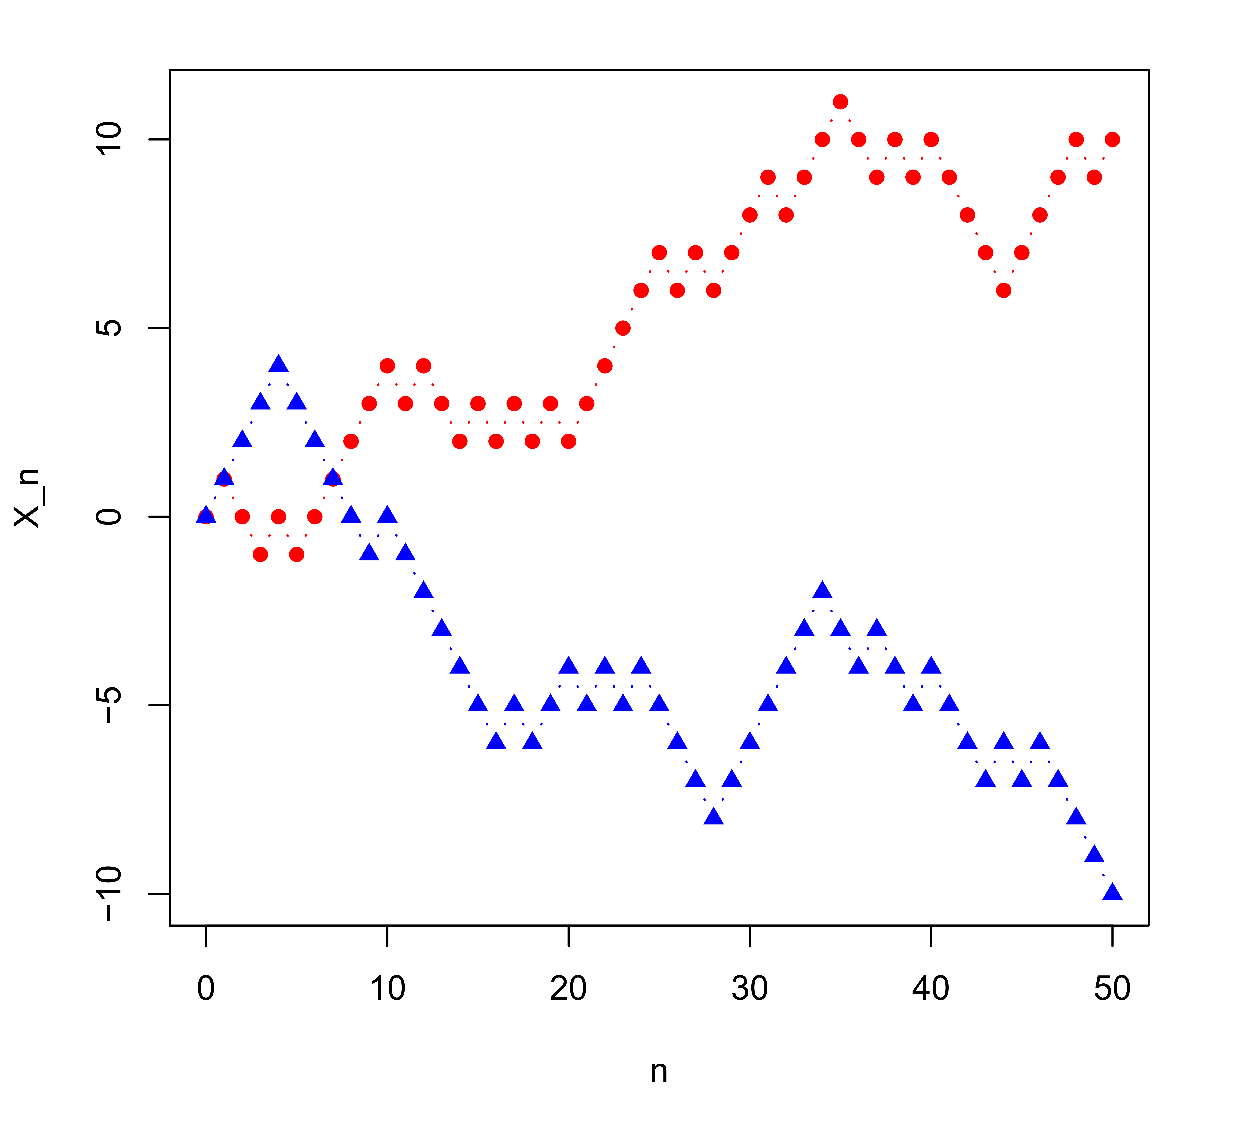
\includegraphics[scale=0.3]{obrazky/random_walk.png}
\caption{Akumulovaný majetek hráče po $k$-té hře, fenomén teplotního šumu}
\end{figure}

Součet nemá Bernoulliho rozložení a nabývá hodnot v oboru celých čísel \textbf{Z}). Definiční vztah lze přepsat

\[ X(k) =X(k-1)+W(k), \]

což je filtr s nekonečnou impulsní odezvou, s pólem $z=1$. Momenty Bernoulliovy řady $\mean{W(k)}=0,\mean{W^2(k)}=1$, momenty náhodné procházky

\begin{eqnarray*}
\mean{X(k)} & = & \mean{\sum W(m)} =  \sum \mean{W(m)} = \sum 0 = 0\\
\mean{X^2(k)} & = & \mean{\left(\sum_{m=1}^k W(m)\right)\cdot\left(\sum_{n=1}^k W(n)\right)}=\\
& = & \mean{\sum_m^k\sum_n^k W(m)W(n)}=\\
& = & \sum^{k,k}_{\substack{m,n\\m\neq n}}\underbrace{\mean{W(m)}}_0 \underbrace{\mean{W(n)}}_0+K = K
\end{eqnarray*}

Platí $\var{X(k)}= \mean{X^2(k)} - \mean{X(k)}^2 = \mean{X^2(k)} - 0^2 =  K$. Variance roste lineárně, proces není stacionární. Autokorelační funkce je ve tvaru

\begin{eqnarray*}
R_{xx}(k_1,k_2) &=& \mean{X(k_1)\cdot X(k_2)}=\mean{\left(\sum_{m=1}^{k_1}W(m)\right)\left(\sum_{n=1}^{k_2}W(n)\right)}=\text{momenty}=\\
& = & \min(k_1,k_2)
\end{eqnarray*}

Pokud to $W(k)$ je Bernoulliho řada bez symetrických hodnot s $ \brs{0,1} $ pak neříkáme Bernoulliho procházka, ale binomická sčítací řada.

\section{Wienerův proces}
Wienerův proces je model fyzikálního jevu známého jako Braunův pohyb, kde se částice chaoticky pohybuje v kapalině díky náhodným srážkám s molekulami kapaliny. Wienerův proces lze odvodit z Bernoulliho řady, která nabývá hodnot $\brs{-\varepsilon,\varepsilon}$ pro malé $\varepsilon>0$. Předpokládejme, že se kolize odehrávají s rychlostí $\alpha$, tzn. odehrávají se v násobcích $\frac{1}{\alpha}$. Celkový počet kolizí za čas $t$ je $n=\lfloor\alpha\cdot t\rfloor$ (zaokrouhlování dolů na celá čísla).

\subsubsection*{Definujeme náhodný proces}
\[ X(t)=\sum_{m=1}^{\lfloor\alpha\cdot t\rfloor} W(m), \]

který je podobný Bernoulliho náhodné procházce, ale

\begin{enumerate}[label=\roman*)]
\item intervaly mezi událostmi jsou $\frac{1}{\alpha}$ namísto 1.
\item amplitudy jsou $\brs{-\varepsilon,\varepsilon}$ namísto $\brs{-1,1}$
\item horní mez je $\lfloor\alpha\cdot t\rfloor$ namísto $k$
\end{enumerate}

Wienerův proces se získá limitním přechodem $\varphi\to 0$ (spojitý náhodný proces) a $\frac{1}{\alpha}\to 0$ (proces spojitý v čase).

\[ Y(t) = \lim_{\substack{\varepsilon\to 0\\ \frac{1}{\alpha}\to 0}} X(t) \]

Jak budou vypadat momenty po limitním přechodu:

\[ \mean{Y(t)} = \lim_{\substack{\varepsilon\to 0\\ \frac{1}{\alpha}\to 0}} \mean{X(t)}=0 \]

Z toho plyne, že Wienerův proces má trvale nulovou střední hodnotu. V případě variace

\[ \mean{Y^2(t)} = \lim_{\substack{\varepsilon\to 0\\ \frac{1}{\alpha}\to 0}} \mean{X^2(t)}=\lim_{\substack{\varepsilon\to 0\\ \frac{1}{\alpha}\to 0}} \lfloor\alpha t\rfloor \varepsilon^2 \]

pro $\frac{1}{\alpha}\to 0, \lfloor\alpha t\rfloor=\alpha t$. Vztah upravíme vytknutím $t$ a tedy

\[ \mean{Y^2(t)} = t \lim_{\substack{\varepsilon\to 0\\ \frac{1}{\alpha}\to 0}} \frac{\varepsilon^2}{\frac{1}{\alpha}} \]

Aby měl proces smysl, musí $\mean{Y^2(t)}>0$ a zároveň $\mean{Y^2(t)}<\infty$. Proto musí $\frac{1}{\alpha}\to 0$ a $\varepsilon^2\to 0$ řádově stejně rychle.

\subsection{Definice Wienerova procesu}
Wienerův proces je náhodný proces spojitý v čase popsaný gaussovskou hustotou pravděpodobnosti, nebo:

\[ P_{x(t)}(x)=\frac{1}{\sqrt{2\pi\alpha\varepsilon^2 t}}e^{-\frac{x^2}{2\alpha\varepsilon^2 t}}, \]

která má nulovou střední hodnotu a varianci $\sigma^2_\lambda(t) = \alpha\varepsilon^2 t$. Počáteční podmínka Wienerova procesu je $P(X(t)=0)=1$. Je to proces spojitý v čase a v úrovni. Odpovídá výstupu integrátoru. Korelační a autokovarianční funkce jsou stejné z důvodu 0 středních hodnot, tedy

\begin{eqnarray*}
R_{xx}(t_1,t_2) &=&\mean{X(t_1)X(t_2)} = \mean{X(t_1)\cdot[X(t_1)+X(t_2)-X(t_1)]} = \\
& = & \mean{X^2(t_1)} + \mean{X)t_1)\cdot(\underbrace{X(t_2)-X(t_1)}_{\text{nezávislý přírůstek}})}= \\
& = & \mean{X^2(t)}+\underbrace{\mean{X(t_1)}}_0\cdot \underbrace{\mean{X(t_2)-X(t_1)}}_0 = \alpha\varepsilon t_1
\end{eqnarray*}

Předpokladem je $t_1<t_2$
\chapter{Úvod do teorie stochastických systémů}
\section{Teorie systémů}
Smyslem vědy je zkoumání dějů, probíhajících v objektech reálného světa, s cílem najít a využít zákonitosti, jimiž se vývoj řídí. K teorii systémů existují dva přístupy, mechanistický a obecný přístup.

\begin{description}
\item[Mechanistický přístup --]
Definice podle Galilea, Newtona a Descarta: Děje lze interpretovat jako soubor určitých elementárních jevů nezávislých na svém okolí (systém je vůči okolí izolovaný). Tento pohled však nebyl schopen řešit řadu významných problémů.

\item[Darwinova teorie --] Darwinova práce poukázala na nezastupitelnou roli náhody a na nutnost zkoumat elementární děje společně s ději, s nimiž \textbf{interagují}.

\item[Obecná teorie --] Nový pohled představovala obecná teorie systémů biologa Ludwig von Bertalanffyho a podobně také Norberta Wienera.
\end{description}

Teorie systémů vychází z předpokladu, že zákonitosti přírodních dějů lze zkoumat jen v souborech všech vzájemně působících dějů. Zkoumají-li se vybrané děje (klíčové/primární), je nutné zkoumat i další děje, které jsou s primárními v interakci.

\subsection{Atributy a vlastnosti systému}
Přírodní děje probíhající na hmotných objektech lze charakterizovat jedním či několika \textbf{atributy}. Ty se mění v čase, přičemž děje jsou tvořeny právě průběhy těchto atributů. Souhrn všech hmotných předmětů, na kterých děje probíhají (primární i interagující) nazveme \textbf{reálným systémem}. Množina tvrzení o vlastnostech systému je pak \textbf{teorie daného systému}.

\tab Vlastnosti systému jsou charakterizovány vlastnostmi časových atributů. Pro vytvoření modelu systému potřebujeme model reálného času a model atributů. Pro jednoduchost vyjdeme z předpokladu, že systém pracuje v diskrétních časových okamžicích a atributy nabývají konečného počtu. Modelem reálného času bude množina $T=\brs{\vecrow[t]}$ s úplným uspořádáním $t_i < t_j$ pro $i < j$.

\begin{note}{Příklad}
Mějme reálný objekt -- vypínač elektrického obvodu. Atributem je stav vypínače (zapnuto - $z$, vypnuto - $v$), modelem bude proměnná $a_1$ a $S_1=\brs{z,v}$. Model je charakterizován několika atributy

\begin{eqnarray*}
\vec{a} & = & [\vecrow[a]]\\
S & = & S_1\times S_2 \times \ldots \times S_n
\end{eqnarray*}

V každém časovém okamžiku nabývá atribut pouze jedné hodnoty. Model průběhu atributů představuje \textbf{trajektorii systému}. Trajektorie je zobrazení z množiny $T$ do množiny $S$, tedy množina trajektorií $\Omega = \brs{s | \, s:T\to S}$, neboli

\[ \vec{s} = [s(t_0), s(t_1), \ldots, s(t_M)]=[s_0,s_1,\ldots, s_M] \]

Reálné děje jsou charakterizovány souhrny trajektorií, jejichž modelem je podmnožina $A\subset\Omega$ a nazývá se \textbf{jevem systému}. Množina všech jevů tvoří algebru jevů $\mathscr{F}$. Jevy mají pravděpodobnostní vlastnosti -- ke každému jevu $A\subset \Omega$ existuje pravděpodobnost $P(A)$, tedy zobrazení $P:\mathscr{F}\to\mathbb{R}$ vyhovující axiomům pravděpodobnosti.
\end{note}

\section{Kauzální stochastický systém}
Stochastický systém lze definovat uspořádanou trojicí

\[ \Sigma = (T,S,P), \]

kde $T$ představuje množinu časových okamžiků, $S$ množinu hodnot atributů a $P$ zobrazení $P:\mathscr{F}\to\mathbb{R}$. Pro teorii stochastických systémů je důležité vedle pravděpodobnostních vlastností trajektorií charakterizovat příčinné vztahy mezi proměnnými systému. Příkladem mohou být následující dvě rovnice

\begin{eqnarray}
y & = & 3x + w\label{eq:sts1}\\
x_{k+1} & = & 3x_k + w_k\label{eq:sts2}
\end{eqnarray}

U první rovnice (\ref{eq:sts1}) není jasné, co nastalo dříve, neboť rovnice nám dává pouze znalost toho, že platí rovnost. U druhé rovnice (\ref{eq:sts2}) je už přidáním indexů zřejmé, která proměnná kdy nastala. Tyto příčinné vztahy se řídí principem kauzality, který říká, že každý jev má svou příčinu. Zobrazení $P$ není nutno vzhledem k axiomatice teorie definovat na celé množině, stačí vymezit vhodné parciální (částečné) zobrazení.

\tab Konkrétní výběr parciálního zobrazení nemá vliv na $P$, ale může reprezentovat další vlastnosti systému. Jím definované pravděpodobnosti budeme nazývat \textbf{kauzálními pravděpodobnostmi}. Ostatní pravděpodobnosti budou pravděpodobnostmi odvozenými. Platí tedy

\[ P(s_0, s_1,\ldots, s_M) = \prod_{k=0}^M P^i(s_{i_k}|s_{i_{k-1}},\ldots, s_{i_0}), \]

kde $i$ je libovolná permutace množiny $[0,1,\ldots, M], i=[i_0,i_1,\ldots, i_M]$.

\begin{note}{Příklad}
Pro $M=2$ máme pravděpodobnost

\begin{eqnarray*}
P(s_0,s_1,s_2) & = & P(s_0|s_1,s_2)\cdot P(s_1|s_2)\cdot P(s_2)\\
& = & P(s_0|s_1,s_2)\cdot P(s_2|s_1)\cdot P(s_1)\\
& = & P(s_1|s_0,s_2)\cdot P(s_0|s_2)\cdot P(s_2)\\
& \vdots &
\end{eqnarray*}
\end{note}

Pravděpodobnostní vlastnosti systému lze charakterizovat pravděpodobnostmi podmíněnými. Dle principu kauzality následek nemůže předcházet příčině, zvolíme tedy identickou permutaci

\[ i_k=k \]

Stochastický systém je definován podmíněnými pravděpodobnostmi

\begin{equation}
P(s_k|s_{k-1},\ldots,s_0)\quad \text{pro } k=1,\ldots,M\label{eq:ppSSP}
\end{equation}

Ty vedle pravděpodobnostních vlastností definují kauzální determinaci řetězce hodnot systémových proměnných. Podmíněné pravděpodobnosti (\ref{eq:ppSSP}) nazveme \textbf{kauzálními pravděpodobnostmi}. Nejprve je dle $P(s_0)$ determinována $s_0$, potom dle $P(s_1|s_0)$ je determinována $s_1,\ldots$ až v čase $k=1,\ldots,M$ je determinována $s_M$ dle

\[ P(s_M|s_{M-1},\ldots,s_0) \]

Kauzální stochastický systém je stochastický systém s vymezenými kauzálními pravděpodobnostmi. Požadavky kladené na atributy vychází z přístupu k teorii systémů.

\begin{enumerate}[label=\alph*)]
\item \textbf{fenomenologická teorie}\\
Tato teorie si všímá zjevných (fenomenologických) atributů. Mějme systém

\[ \Sigma = (T,S,P^1), \]

kde $P_1$ je množina zobrazení $P_k, k=0,1,\ldots, M$, které definují kauzální pravděpodobnosti. Systémová proměnná $s_k$ v čase $k$ je obecně determinována celou historií systému vyjádřenou posloupností

\[ s_{k-1},s_{k-2},\ldots,s_0 \]

\item \textbf{stavová teorie}\\
Atributy systému jsou v každém časovém okamžiku charakterizovány souborem tzv. stavových proměnných, který má všechny vlastnosti proměnných fenomenologické teorie a navíc v souboru stavových proměnných dochází k \textit{působení minulosti na budoucnost pouze prostřednictvím přítomnosti}. Soubor stavových proměnných je zpravidla rozsáhlejší, než soubor proměnných fenomenologických. Mějme systém

\[ \Sigma = (T,S,P^1) \]

Pro kauzální pravděpodobnosti však platí

\[ P(s_k|s_{k-1},s_{k-2},\ldots,s_0) = P(s_k|s_{k-1}), k =0,1,\ldots,M \]

Rozšíření $S$ na nespočetné množiny je triviální a podmíněné pravděpodobnosti se nahradí podmíněnými hustotami pravděpodobnosti. Pro střední hodnotu platí

% \[ \mean{\d W\quad \d W\t} = Q\d t, \]
%
% kde $\d W$ lze interpretovat jako $W(t+\d t) - W(t)$
\end{enumerate}

\subsection{Příklady stochastických systémů}
\begin{itemize}
\item \textbf{Systémy s diskrétním časem a spojitými stavy}, pro které je množina časových okamžiků $T = \brs{t_0,t_1,\ldots, t_M}, S=\mathbb{R}^n$, $\mathscr{F}$ je borelovská $\sigma$-algebra na $S\t$ a hustota pravděpodobností $p(s_k|s_{k-1})$ pro $k=1,2,\ldots,M$ vyjadřující závislost pouze do současnosti ($k-1$), na rozdíl od fenomenologické teorie (tam jsou prvky podmíněné hustoty až do prvku $s_0$).

\item \textbf{Stochastické diferenční rovnice} představují alternativní popis místo hustoty $p(s_k|s_{k-1})$ ve tvaru

\[ s_{k+1}=F_k(s_k,\xi_k),\quad k=0,1,\ldots, M-1 \]

s počáteční podmínkou $p(s_0)$ a $\brs{\xi_k, k=0,1,\ldots,M-1}$ posloupností nezávislých náhodných veličin s daným rozdělením pravděpodobnosti (tedy náhodný proces). Hustotu $p(s_k|s_{k-1})$ lze z této stochastické diferenční rovnice určit.

\item \textbf{Stochastické diferenciální rovnice} představuje tzv. Itô-ova stochastická diferenciální rovnice $T=\mathbb{R}^+$ ve tvaru

\[ \d s(t) = F\big(s(t),t\big)\d t + G\big(s(t),t\big)\d W(t), \]

kde $F\big(s(t),t\big)$ je náhodná funkce, $G\big(s(t),t\big)$ představuje obecně maticový koeficient a $W(t)$ je Wienerův proces. Rovnice je zapsána pouze pomocí diferenciálů, neboť derivace Wienerova procesu $\frac{\d}{\d t} W(t)$ neexistuje!
\end{itemize}

Pro formální derivace náhodného procesu $\brs{w(t), t\geq t_0}$ platí, že má nulovou střední hodnotu a formální kovarianční matici

\[ C_{ww}(t,\tau)=Q\sigma(t-\tau), \]

kde $\sigma$ značí Diracův pulz. Pro $Q$, resp. $G$ nulové přejde stochastický diferenciální rovnice v obyčejnou (deterministickou) rovnici

\begin{eqnarray*}
\d s(t) & = & F\big(s(t),t\big)\d t\\
\dot{s}(t) & = & F\big(s(t),t\big)
\end{eqnarray*}

Řešení takové stochastické rovnice je ve tvaru

\[ s(t) = s(t_0) + \int\limits_{t_0}^t F\big(s(\tau\big)\tau)\d\tau + \int\limits_{t_0}^t G\big(s(\tau,\tau\big)\d W(\tau), \]

kde první integrál je Riemannův integrál a druhý Itô-ovův stochastický integrál.
\chapter{Průchod signálu lineárním stavovým systémem}
\section{Deterministický stavový model}
Deterministický stavový model lineárního diskrétního systému

\begin{eqnarray*}
x_{k+1} & = & Ax_k + Bu_k\\
y_k & = & Cx_k + Du_k,
\end{eqnarray*}

kde $x_{k+1}=x(t_{k+1})$ a počátečním stavem $x_0$. Na základě znalosti stavu systému a modelu můžeme přesně určit příští stav systému a jeho výstup. V mnoha případech je tento způsob popisu nedostatečný, určitá složka výstupu nemusí být přesně predikovatelná. Z toho vyplývá, že je nutné popsat signály jako náhodné procesy.

\tab Do systému si tedy zavedeme další dva vstupy a dostaneme \textbf{lineární stochastický systém} (resp. model stochastického diskrétního systému).

\begin{eqnarray*}
x_{k+1} & = & Ax_k + Bu_k + w_k\\
y_k & = & Cx_k + Du_k + v_k,
\end{eqnarray*}

kde $u_k$ je deterministický vstup, $w_k, v_k$ jsou stacionární náhodné posloupnosti, které nazýváme šum systému ($w_k$ -- šum procesu (stavu), $v_k$ -- šum měření). Předpokládáme, že posloupnosti tvoří nezávislé náhodné posloupnosti se stejným rozdělením pravděpodobnosti. Dále předpokládáme, že jsou nezávislé na minulých hodnotách vstupu a stavu.\br

Předpokládejme, že oba dva vstupy mají nulovou střední hodnotu, tj.

\[ \mean{
\begin{bmatrix}
w_k \\ v_k
\end{bmatrix}
} = 0 \]

a 

\[
\mathrm{cov}\left\{ \begin{bmatrix}w_k \\ v_k\end{bmatrix},\begin{bmatrix}w_e \\ v_e\end{bmatrix} \right\}
=\mean{ \begin{bmatrix}w_k \\ v_k\end{bmatrix} \cdot \begin{bmatrix}w_e \\ v_e\end{bmatrix}\t  } =
\begin{bmatrix}
Q & S\\ S\t & R
\end{bmatrix}\cdot\delta(k-e)
\]

\[ \delta(k-e)=\begin{cases} 1 & \text{pro } k = e\\ 0 & \text{jinak} \end{cases} \]

náhodný proces s těmito vlastnostmi nazýváme \textbf{bílý šum}. Jak se vyvíjí stav a výstup systému? Omezíme se na popis střední hodnoty a vzájemné (auto)kovarianční funkce. Zavedeme značení

\[ m_k^x=\mean{x_k}, m_k^y=\mean{y_k} \]

\begin{eqnarray*}
\mean{x_{k+1}} & = & \mean{Ax_k+Bu_k+w_k} =\\
& = & A\mean{x_k}+Bu_k \Rightarrow m_{k+1}^x = Am_k^x + Bu_k\\
&&\\
\mean{y_k} & = & \mean{Cx_k+Du_k+v_k} =\\
& = & C\mean{x_k}+Du_k \Rightarrow m_{k}^y = Cm_k^y + Du_k
\end{eqnarray*}

Střední hodnota se vyvíjí stejně, jako stav deterministického systému. Označme odchylky od střední hodnoty $\widetilde{x}_k = x_k-m_k^x$, resp. $\widetilde{y}_k=y_k-m_k^y$ a zaveďme

\[ P_k^x=\mathrm{cov}[x_k]=\mean{\widetilde{x}_k\, \widetilde{x}_k\t} \]

Odečtením rovnic získáme stavový popis

\begin{eqnarray*}
\widetilde{x}_{k+1} & = & A\widetilde{x}_k + w_k\\
\widetilde{y}_l & = & C\widetilde{x}_k + v_k,
\end{eqnarray*}

ted $\widetilde{x}_{k+1}\widetilde{x}_{k+1}\t = A\widetilde{x}_{k}\widetilde{x}_{k}\t A\t + A\widetilde{x}_{k}w_k\t + w_k\widetilde{x}_{k}\t A\t+w_kw_k\t$.

\[ \mean{\widetilde{x}_{k+1}\, \widetilde{x}_{k+1}\t} = A\mean{\widetilde{x}_{k}\,\widetilde{x}_{k}\t}A\t=Q \]

To lze zapsat jako

\[ P_{k+1}^x = AP_k^x A\t+Q \]

$\widetilde{x}_{k+1}\widetilde{y}_{k}\t = A\widetilde{x}_{k}\widetilde{x}_{k}\t C\t + A\widetilde{x}_{k}v_k\t + w_k\widetilde{x}_{k}\t C\t+w_k v_k\t$. Střední hodnota je

\[ \mean{\widetilde{x}_{k+1}\, \widetilde{y}_{k}\t} = AP_k^x C\t + S \]

Jako poslední možnost jsou $\widetilde{y}_{k}\widetilde{y}_{k}\t = C\widetilde{x}_{k}\widetilde{x}_{k}\t C\t + C\widetilde{x}_{k}v_k\t + v_k\widetilde{x}_{k}\t C\t+v_k v_k\t$, jehož střední hodnota je 

\[ \mean{\widetilde{y}_{k}\, \widetilde{y}_{k}\t} = CP_k^x C\t + R \]

Rovnice pro sdruženou kovarianční matici stavu a výstupu

\[
\mathrm{cov}\left\{ \begin{bmatrix}x_{k+1} \\ y_k\end{bmatrix} \right\} =
\begin{bmatrix}
AP_k^x A\t+Q & AP_k^x C\t + S\\
CP_k^x A\t + S\t & CP_k^x C\t + R
\end{bmatrix}
\]

Podobně vztahy pro autokovarianční funkci stavu

\[ C_{xx}(k,e) = \mean{\widetilde{x}_k\, \widetilde{x}_e\t}=A^{k-e}P_e^x+Q\delta(k-e), k>e \]

a autokovarianční funkce výstupu

\[ C_{yy}(k,e) = CA^{k-e}P_e^x C\t + R\delta(k-e) + CA^{k-e-1}S(1-\delta(k-e)), k\geq e \]

Jsou-li $w_k$ a $v_k$ gaussovské a $x_0$ také gaussovský, charakterizují první dva momenty stavu a výstupu jejich rozložení, které je také gaussovské. Pokud je počáteční podmínka $x_0$ popsaná prvníma dvěma momenty $m_0^x$ a $P_0^x$, lze $m_k^x$ a $P_k^x$ vyjádřit explicitně.

\[ m_k^x = A^k m_0^x+\sum_{j=0}^{k-1}A^{k-j-1}Bu_j \]

\[ P_k^x = A^k P_0^x (A^k)\t+\sum_{j=0}^{k-1}A^j Q (A^j)\t \]

Je-li $A$ stabilní, pak řada pro kovarianční matici konverguje a lze nalézt ustálené řešení

\[ P^x = \lim_{k\to\infty} P_k^x \]

které vyhovuje Ljapunovové rovnici

\[ P^x = AP^xA\t + Q \]

Ustálená hodnota kovariančního výstupu pak je

\[ P^y = CP^x C\t + R \]
\chapter{Průchod signálu LDS ve fenomenologickém popisu}
Budeme charakterizovat vlastnosti náhodných signálů po průchodu lineárním dynamickým systémem (LDS) definovaným vnějším popisem. Pro jednoduchost budeme uvažovat jednorozměrný systém (kauzální) popsaný impulsní charakteristikou $g_k$($g_k=0$ pro $k<0$). Vstupem systému bude náhodný proces (posloupnost) $u_k$ s konečnými druhými momenty. Střední hodnotu označíme $\mean{u_k}=m_k^u$ s autokovarianční funkcí

\[ C_{uu}(k,e) = \mean{(u_k-m_k^u)(u_e-m_e^u)} \]

pro výstup platí

\[ y_k = \sum_{l \to \infty}^k g_{k-l}u_e=\sum_{l=0}^{\infty} g_l u _{k-l} \]

Pro stabilní systém řada konverguje (\uv{ve středně-kvadratickém smyslu}) a výstup $y_k$ je zase náhodná posloupnost s konečými druhým momenty

\[ m_k^y = \mean{y_k}=\mean{\sum_{l=0}^\infty g_l u_{k-l} } = \sum_{l=0}^\infty g_lm_{k-l}^u \]

Pro výpočet autokovarianční funkce si definujeme odchylky $\widetilde{u}^k=u_k-m_k^u$ a $\widetilde{y}_k=y_k-m_k^u$, pro které platí

\[
\widetilde{y}_k = y_k-m_k^y = \sum_{l=0}^\infty g_l u_{k-l}-\sum_{l=0}^\infty g_l m_{k-l}^u=\sum_{l=0}^\infty g_l \widetilde{u}_{k-l}
\]

Rozdíl mezi signálem a jeho střední hodnotou se filtruje stejně, jako střední hodnota. Autokovarianční funkce výstupu pak bude

\begin{eqnarray*}
C_{yy}(k,l) &=& \mean{\widetilde{y}_k\, \widetilde{y}_l}=\mean{ \sum_{i=0}^\infty g_i \widetilde{u}_{k-i}\cdot \sum_{j=0}^\infty g_j\widetilde{u}_{l-j} } = \\
& = & \sum_{i=0}^\infty \sum_{j=0}^\infty g_i g_j\mean{\widetilde{u}_{k-i}\, \widetilde{u}_{k-j}} = \\
& = & \sum_{i=0}^\infty \sum_{j=0}^\infty g_i g_j C_{uu}(k-i,l-j)
\end{eqnarray*}

Podobně vzájemná autokovarianční funkce mezi výstupem $y_k$ a vstupem $u_k$.

\begin{eqnarray*}
C_{yu}(k,l) &=& \mean{\widetilde{y}_k\, \widetilde{u}_l}=\mean{ \sum_{i=0}^\infty g_i \widetilde{u}_{k-i}\cdot \widetilde{u}_l } = \\
& = & \sum_{i=0}^\infty g_i\mean{\widetilde{u}_{k-i}\, \widetilde{u}_{l}} = \\
& = & \sum_{i=0}^\infty g_i  C_{uu}(k-i,l)
\end{eqnarray*}

Je-li vstupní proces gaussovský, je i výstupní proces gaussovský (jenom tranformujeme náhodné veličiny, vynásobíme konstantou a sečteme, proto zůstane g. proces gausovský). Zjednodušení výsledků, pokud bude vstupní proces stacionární, tedy


Autokovarianční funkce výstupu

\[ C_{yy}(k,e) = \sum_{i=0}^\infty \sum_{j=0}^\infty g_i g_j C_{uu}(k-e+j-i)=C_{yy}(k-e) \]

Vzájemná autokovarianční funkce výstupu a vstupu

\[ C_{yu}(k,e) = \sum_{i=0}^\infty g_i C_{uu}(k-e-j)=C_{yu}(k-e) \]

Střední hodnota výstupu je konstantní (nemění se v čase), obě autokovarianční funkce jsou funkcí rozdílu časových okamžiků. Výstupní proces je tedy stacionární v širším smyslu a výstup a vstup jsou vzájemně stacionární.

\[ m_k^u = m^u, C_{uu}(k,l)=C_{uu}(k-l) \]

 Lze psát, rovnice pro střední hodnotu

kde
\[ K=\sum_{i=0}^\infty g_i \]

střední hodnota

\[ m_k^y\]


\[ C_{yy}(k,l) = \sum_{i=0}^\infty \sum_{j=0}^\infty g_i g_j C_{uu}(k-i-j)= C_{yy}, \]

vzájemná kovarianční funkce

\[ C_{yu}(k,l) = \sum_{i=-0}^\infty g_i C_{uu}(k-i-l)=C_{uu}(k-l), \]


střední hodnota výstupu je konstantní, obě autokovarianční fce jsou funkcemi č. okamžiků, tj. výstup je staionární v šírším smyslu a vstup a výstup jsou vzájemně stacionární



někdy se zapisují pomocí konvolutorního operátoru $*$ je, vzájemná autokovarianční funkce je konvolucí impulsní funkce a autokovarianční funkce vstupu.

\[ C_{yu} (k)  =\sum_{i=-\infty}^\infty g_i C_{uu} (k-i) = g * C_{uu} \]

vzájemná kovarianční funkce výstupu a vstupu je konvolucí impulsní funkce a autokovarianční funkce vstupu.

Obdobně to můžeme udělat pro autokovarianční funkci výstupu

\[ C_{yy} (K) = \sum_{i=-\infty}^\infty \sum_{j=-\infty}^\infty g_i g_j C_{uu} (k+j-i) = \sum_{i=-\infty}^\infty \sum_{j=-\infty}^\infty g_i C_{uu}(k-j-i) g_{-j} = g * C_uu * \bar{g}   \]

kde $\bar{g}_k=g_{-k}$,

\uv{To je jen šikovný zápis :)}
\chapter{Spektrální faktorizace diskrétního náhodného procesu}
Stejně jako u lineárních t-invariantních deterministických systémů lze vztahy mezi vstupy a výstupy popisovat ve frekvenční oblasti. Označíme

\[ G(z) = \sum_{i=0}^\infty g_iz^{-i} \]

Tato rovnice vyjadřuje přenos v Z-transformaci. Definujeme spektrální hustotu procesu jako Z-transformaci autokovarianční (popřípadě vzájemné kovarianční) funkce vyčíslené v jednotkové kružnici.

\[ z=e^{j\omega T_s},\quad \omega\in(-\omega_n,\omega_n), \]

kde $\omega_n$ je tzv. Nyquistova frekvence $\omega_n = \frac{\pi}{T_s}$. Označme

\begin{alignat*}{2}
S_{uu}(\omega) & = S_{uu}(z)|_{z=e^{j\omega T_s}}, S_{uu}(z) && = \sum_{i=-\infty}^\infty C_{uu}(i)z^{-i}\\
S_{yy}(\omega) & = S_{yy}(z)|_{z=e^{j\omega T_s}}, S_{yy}(z) && = \sum_{i=-\infty}^\infty C_{yy}(i)z^{-i}\\
S_{yu}(\omega) & = S_{yu}(z)|_{z=e^{j\omega T_s}}, S_{yu}(z) && = \sum_{i=-\infty}^\infty C_{yu}(i)z^{-i}
\end{alignat*}

Tato definice spektrální hustoty odpovídá formálně Fourierově transformaci (auto) kovarianční funkce. Platí:

\begin{eqnarray*}
S_{yu}(z) & = & \sum_{i=-\infty}^\infty C_{yu}(i)z^{-i} = \sum_{i=-\infty}^\infty z^{-i} \sum_{j=0}^\infty C_{uu}(i-j) = \sum_{i=-\infty}^\infty \sum_{j=0}^\infty z^{-i} g_j C_{uu}(i-j) = \\
& = & \sum_{i=-\infty}^\infty \sum_{j=0}^\infty z^{-j} g_j z^{-(i-j)} C_{uu}(i-j) = \sum_{j=0}^\infty z^{-j}g_j \sum_{i=-\infty}^\infty z^{-(i-j)} C_{uu}(i-j) =
\end{eqnarray*}

Odtud platí

\[ S_{yu}(z) = G(z)\cdot S_{uu}(z) \]

neboli

\[ S_{yu}(\omega) = G\left(e^{j\omega T_s}\right)\cdot S_{uu}(\omega) \]

Pro opačné pořadí vstupu a výstupu platí

\[ S^{uy}(z) = S_{uu}(z)\cdot G^*(z), \]

kde $G^*(z)=G(z)|_{z=z^{-1}}$, tedy

\[ S_{uy}(\omega) = S_{uu}(\omega)\cdot G^*\left(e^{j\omega T_S}\right)  \]

Pro spektrální hustotu výstupu platí

\[ S_{yy}(z) = \sum_{i=-\infty}^\infty z^{-i}C_{yy}(i) = \cdots = \sum_{j=0}^\infty z^{-j}g_j \sum_{i=-\infty}^\infty z^{-i} C_{uu}(i)\sum_{k=0}^\infty z^{-k}g_k \]

tedy

\begin{eqnarray*}
S_{yy}(z) & = & G(z)\cdot S_{uu}(z)\cdot G^*(z)\\
S_{yy}(\omega) & = & \left(G\left(e^{-j\omega T_s}\right)^2\right)\cdot S_{uu}(\omega)
\end{eqnarray*}

\subsection{Fyzikální interpretace}
Protože 

\[ \frac{1}{2\omega_n}\int\limits_{-\omega_n}^{\omega_n}S_{uu}(\omega)\d\omega = C_{uu}(0)=\delta_u^2=\mean{u_k^2} \]

Je měřítkem výkonu procesu, lze hodnotu (výkonové) spektrální hustoty v bodě $\omega$ chápat jako hustotu výkonu v okolí frekvence $\omega$. Součin

\[ G\left(e^{j\omega T_s}\right)\cdot G\left(e^{-j\omega T_s}\right) = \left|G\left(e^{j\omega T_s}\right)\right|^2 \]

udává výkonové zesílení na této frekvenci a hodnota $S_{yy}(\omega)$ je pak hustota výkonu výstupního signálu v okolí této frekvence.

\section{Využití vztahů pro vzájemnou autokovarianční funkci a vzájemnou spektrální hustotu pro identifikaci systému}

Uvažujme jako vstupní proces diskrétní bílý šum s autokovarianční funkcí

\[ C_{uu}(k) = \delta(k), \]

kde $\delta$ je Diracův impuls a spektrální hustotou

\[ S_{uu}(z) = \sum_{i=-\infty}^\infty C_{uu}(i)z^{-i} = \sum_{i=-\infty}^\infty \delta(i)z^{-i}=z^0=1 \]

Pro tento vstup získáme 

\begin{eqnarray*}
C_{yu}(k) & = & \sum_{i=-\infty}^\infty g_iC_{uu}(i-k) = \sum_{i=-\infty}^\infty g_i\delta(k-i)=g_k\\
S_{yu}(\omega) & = & G\left(e^{-j\omega T_s}\right)\cdot S_{uu}(\omega) = G\left(e^{j\omega T_s}\right)
\end{eqnarray*}

Vzájemná autokovarianční funkce je tedy rovna impulsní charakteristice systému a vzájemná spektrální hustota je rovna jeho frekvenčnímu přenosu.

\section{Spektrální faktorizace diskrétního náhodného procesu}

Kovarianční matice a spektrální události náhodného procesu závisí pouze na odchylkách uvažovaných signálů. Budeme uvažovat nulový deterministický vstup $u$ a vstupem budou pouze bílé šumy $w$ a $v$. Popis systému:

\begin{eqnarray*}
x_{k+1} & = & \vec{A}x_k + w_k\\
y_k & = & \vec{C}x_k + v_k
\end{eqnarray*}

pokud je $A$ stabilní, po uplynutí dostatečně dlouhé doby od $k=0$ budou stav i výstup stacionární náhodné procesy s nulovou střední hodnotou. K určení jejich kovarianční matice je nutno řešit Ljapunovovu rovnici a rovnici pro výstup.

\begin{eqnarray*}
P^x & = & \vec{A}P^x\vec{A}\t + \vec{Q}\\
P^y & = & \vec{C}P^x\vec{C}\t + \vec{R}
\end{eqnarray*}

Označme
\[ u_k = 
\begin{bmatrix}
w_k\\v_k
\end{bmatrix}
\]

Potom přenos mezi tímto vstupem a výstupem $y_k$ je

\[ G(z) = [C(zI-A)^{-1}, I] \]

Spektrální hustota vstupu je 

\[ S_{uu}(z) =
\begin{bmatrix}
Q & S\\
S\t & R
\end{bmatrix}
\]

a potom

\[
S_{yu}(z) = [C(zI-A)^{-1}, I]\cdot
\begin{bmatrix}
Q & S\\ S\t & R
\end{bmatrix}
\]

\[ S_{uy}(z) = S\t_{yu}(z) \]

\[ S_{yy}(z) = [C(zI-A)^{-1}, I]\cdot 
\begin{bmatrix}
Q & S\\ S\t & R
\end{bmatrix}\cdot [C(zI-A)^{-1}, I]\t
\]

Pro vzájemně nezávislé šumy $w_k$ a $v_k$ s kovarianční maticí

\[ \mathrm{cov}\left\{ \begin{bmatrix} w_k\\v_e \end{bmatrix}, \begin{bmatrix} w_e\\ v_e \end{bmatrix} \right\} = \mean{\begin{bmatrix} w_k\\v_e \end{bmatrix}\cdot \begin{bmatrix} w_e\\ v_e \end{bmatrix}\t} = \begin{bmatrix}
Q & 0 \\ 0 & R
\end{bmatrix}\delta(k-e) \]

Bude platit

\[ S_{yy}(z) = C(zI-A)^{-1}\cdot Q(zI-A)^{-\mathrm{T}}C\t + R \]

\begin{note}{Příklad rozkladu spektrální hustoty}
Uvažujme spektrální hustotu, která je nezápornou racionální funkcí $\cos(\omega T_s)$

\[ S_{yy}(z) = \frac{(z+0.5)(z^{-1}+0.5)}{(z+0.25)(z^{-1}+0.25)} \]

Pro $S_{uu}(\omega) = 1$ platí

\[ S_{yy}(z) = G(z)\cdot S_{uu}(z)\cdot G^*(z) = C(z)\cdot G^*(z),\quad G^*(z)=G(z)|_{z=z^{-1}} \]

Tuto racionální spektrální hustotu lze vyjádřit čtyřmi způsoby:

\begin{alignat*}{2}
G_1(z) & = \frac{z+0.5}{z+0.25} && \to \text{stabilní}\\
G_2(z) & = \frac{1+0.5z}{z+0.25} && \to \text{stabilní}\\
G_3(z) & = \frac{z+0.5}{1+0.25z} && \to \text{nestabilní}\\
G_4(z) & = \frac{1+0.5z}{1+0.25z} && \to \text{nestabilní}
\end{alignat*}

Stochastický signál s danými spektrálními vlastnostmi můžeme získat průchodem bílého šumu dynamickými systémy s přenosy $G_1$ a $G_2$ z nich $G_1$ má minimální fázi. Z toho plyne, že také inverze má stabilní přenos. Takovému rozkladu spektrální hustoty říkáme \textbf{spektrální faktorizace náhodného procesu}.
\end{note}

\subsection{Věta o spektrální faktorizaci}

Předpokládejme, že $S_{yy}(\omega)$ je racionální funkcí $\cos(\omega T_s)$ případně $e^{j\omega T_s}$, pak existuje právě jedna monická (= 1 u nejvyšších mocnin polynomů v čitateli i jmenovateli) racionální funkce $G(z)$, která má všechny póly uvnitř jednotkové kružnice a všechny nuly uvnitř, nebo na jednotkové kružnici. Platí

\[ S_{yy}(\omega) = G^2\left|G\left(e^{j\omega T_s}\right)\right|^2 \]

Uvažujme náhodný proces vzniklý průchodem bílého šumu s rozptylem $\sigma^2$ dynamickým systémem s přenosem $G(z)$ dle předchozí věty. Jeho spektrální hustota pak bude $S_{yy}(z)$.

\subsection{Věta o realizaci}
Pro každou racionální spektrální hustotu $S_{yy}\geq 0$ existuje právě jeden dynamický systém s přenosem $G(z)$, který je monickou racionální funkcí, má všechny póly uvnitř jednotkové kružnice a nuly uvnitř, nebo na jednotkové kružnici takový, že stacionární proces s danou spektrální hustotou můžeme získat jako výstup systému je-li vstupem diskrétní bílý šum.

\subsubsection{Důsledek}
Omezíme-li se na stacionární procesy s racionálními spektrálními hustotami, lze takové procesy získat filtrací diskrétního bílého šumu. Takové náhodné procesy lze reprezentovat ve tvaru:

\[ y_k = \frac{c(d)}{a(d)}e_k, \]

kde $e_k$ je bílý šum s rozptylem $\sigma^2$, $d$ je operátor zpoždění $d\cdot y_k=y_{k-1}$ a $c(d),a(d)$ jsou polynomy:

\begin{eqnarray*}
a(d) & = & 1 + a_1d + \cdots + a_{n_a}d^{n_a}\\
c(d) & = & 1 + c_1d + \cdots + a_{n_c}d^{n_c}
\end{eqnarray*}

nebo v časové oblasti

\[ y_k + a_1y_{k+1}+\cdots+a_{n_a}y_{k-n_a}=e_k+c_1e_{k-1}+\cdots+c_{n_c}e_{k-n_c} \]

Tato reprezentace se nazývá ARMA model (Autoregressive–moving-average model). Podle věty o realizaci lze nalézt polynomy $a(d)$ a $c(d)$ tak, aby byly oba stabilní (kromě kořenů $c(d)$ na jednotkové kružnici). Původní transformaci lze tedy invertovat:

\[ e_k=\frac{a(d)}{c(d)}y_k \]

Posloupnost $\{\ldots, y_{k-1}, y_k \}$ obsahuje veškeré informace o měřené posloupnosti $\{ \ldots, e_{k-1},e_k \}$. Ukážeme si důležitou vlastnost této bílé posloupnosti a zavedeme pojem \textbf{inovace}.

\subsection{Inovační reprezentace}
Uvažujme

\[ y_{k+1}=\frac{c(d)}{a(d)}e_{k-1} \]

a provedeme dělení polynomů

\[ \frac{c(d)}{a(d)} = 1+\frac{d\bar{c}(d)}{a(d)} \]

tedy

\[ y_{k+1} = \frac{\bar{c}(d)}{a(d)}\cdot e_k+e_{k+1} \]

Dosadíme za $e_k$ a dostaneme

\[ y_{k+1} = \frac{\bar{c}(d)}{a(d)}\cdot\frac{a(d)}{c(d)}y_k+e_{k+1}=\frac{\bar{c}(d)}{c(d)}y_k+e_{k+1} \]

Z toho plyne, že hodnotu $e_{k+1}$ můžeme interpretovat jako tu část informace o $y_{k+1}$, která není obsažena v minulé historii procesu $\{ \ldots,y_{k-1},y_k \}$, a proto ji nazýváme \textbf{inovace procesu}. Protože $e_k$ je bílá posloupnost, je $\widehat{y}_{k+1}=\frac{\bar{c}(d)}{c(d)}y_k$ nejlepší predikcí výstupu na základě zadané historie procesu $\{ \ldots, y_{k-1},y_k \}$ ve smyslu střední kvadratické chyby $\mean{(\ldots, y_{k+1}-\widehat{y}_{k+1})^2}$ a reprezentaci

\[ y_k = \frac{c(d)}{a(d)}e_k = \sum_{r=0}^\infty g_r e_{k-r} \]

nazýváme \textbf{inovační reprezentace}.

\begin{note}{Poznámka}
pracujeme-li s inovační reprezentací, tj. vstupní posloupnost je bílá, lze model převést do tvaru prediktoru. Jestliže však vstupní posloupnost není bílá, není $\widehat{y}_{k+1}$ dle předchozího vztahu optimální prediktor, neboť $e_{k+1}$ je korelována s předchozími daty, a proto může být chyba predikce dále zmenšena.
\end{note}

\begin{note}{Příklad - optimální prediktor výstupu}
Uvažujme spektrální hustotu

\[ S_{yy}(z) = \frac{(z+0.5)(z^{-1}+0.5)}{(z+0.25)(z^{-1}+0.25)} \]

Podle věty o realizaci lze tuto hustotu získat průchodem bílého šumu filtrem.

\[ y_k = \frac{1+0.5d}{1+0.25d}e_k,\quad \left(G(z) = \frac{z+0.5}{z+0.25}\right) \]

protože

\[ \frac{1+0.5d}{1+0.25d} = 1+\frac{0.25d}{1+0.25d} \]

lze proces popsat

\[ y_{k+1} = \frac{0.25d}{1+0.5d}y_k+e_{k+1} \]

a optimální prediktor výstupu $y_{k+1}$ je

\[ \widehat{y}_{k+1} = \frac{0.25d}{1+0.5d}y_k \] 

\end{note}

% Cvičení
\part{Praktické úlohy}
\chapter{Pravděpodobnost a míra pravděpodobnosti}
\section{Pravděpodobnostní prostor}
Máme množiny $\Omega$, která představuje množinu \textbf{elementárních} (základních) jevů a množinu $\mathscr{U}$ představující množinu jevů. Dále máme definovánu pravděpodobnostní míru $\mu$.

\begin{note}{Příklad}
Uvedeme si příklad těchto množin na \textbf{hrací kostce}. Máme kostku, kde množina elementárních jevů $\Omega=\{"1","2","3",\ldots,"6"\}$ a množiny jevů $A_1,A_2, \ldots, A_n\in\mathscr{U}$ jsou například:

\begin{itemize}[noitemsep]
\item $A_1=\{"2","4","6"\}$ značící, že na kostce padlo sudé číslo
\item $A_2=\{"1","2"\}$ značící, že na kostce padlo číslo menší než $3$
\item $A_3=\{"3"\}$ značící, že na kostce padlo právě číslo $3$
\end{itemize}
\end{note}

Klasická definice pravděpodobnosti nějakého jevu $A$ se počítá dle vztahu \ref{cv1:eq_defppsti}
\begin{equation}
P(A) = \frac{\text{velikost} A}{\text{velikost} B}\label{cv1:eq_defppsti}
\end{equation}

Tato definice ale není platná v jakémkoliv případě, neboť například u nekonečně veliké množiny $\Omega$ vztah \ref{cv1:eq_defppsti} selže. Proto se \textbf{předpokládá}, že množina $\Omega$ má konečný počet prvků a všechny výsledky experimentu $\omega\in\Omega$ mají stejnou nenulovou pravděpodobnost.

\begin{note}{Příklad}
Pokud budeme tedy například předpokládat hrací kostku s \textbf{pětkou na třech stranách}, jsou pro množinu $\Omega=\{"1","2","3","5"\}$ následující pravděpodobnosti

\[
P(A)=
\begin{cases}
\frac{1}{2} & \text{pro } A=\{5\}\\
\frac{1}{2} & \text{pro } A=\{1\}\vee A=\{2\}\vee A=\{3\}\\
0 & \text{jinak}
\end{cases}
\]

Dalším příkladem může být \textbf{predikce polohy větrné korouhvičky}. Mějme množinu elementárních jevů
\[ \Omega=\{\omega, 0 \si{\degree} <\omega\leq 360 \si{\degree} \}. \]

Množina $\Omega$ je \textbf{nespočetná}! Existuje tedy nekonečně mnoho hodnot $\omega$. Pro jev $A\in\mathscr{U},A=\{\omega,\omega\in\Omega\}$ se nedá definovat pravděpodobnost a je tedy třeba definovat správnou množinu elementárních jevů.
\end{note}

\subsection{$\sigma$-algebra}
Definujeme třídu podmnožin (algebru), která vždy umožní určit pravděpodobnost elementárních jevů a zároveň je dostatečně obecná a aby obsahovala jevy, které si můžeme představit. Algebra $\mathscr{U}$ musí splňovat následující podmínky:

\begin{itemize}[noitemsep]
\item Pokud $A\in\mathscr{U}$, pak i doplněk $A^c\in\mathscr{U}$.
\item Pokud $A,B\in\mathscr{U}$, pak i $A\cup B\in\mathscr{U}$.
\end{itemize}

Třída podmnožin $\Omega$ je tzv. \textbf{$\sigma$-algebra}, pokud je to algebra a navíc pokud společné množiny $A_1,A_2,\ldots, A_n$? jsou v algebře a je tam i jejich sjednocení

\[ A_1,A_2,\ldots,A_n\in\mathscr{U}\to\bigcup_{i=1}^\infty A_i\in\mathscr{U} \]

Nechť $\{\Omega, F\}$ je měřitelný prostor a míra $M$ je funkce, která přiřazuje $F$ nějaké číslo z intervalu $\langle 0, \infty)$ a tato funkce musí splňovat

\begin{enumerate}[label=\alph*)]
\item Míra $M(\emptyset)=0$
\item Pokud jevy $A_i, i=1,2,\ldots,n$ jsou disjunktní, potom
\[ M\left(\bigcup_{i=1}^\infty A_i\right) = \sum_{i=1}^\infty M(A_i) \]
\end{enumerate}

\textbf{Pravděpodobnostní míru} pak nazveme míru, která je normovaná na interval $M:F\to\langle 0, 1\rangle$. Pravděpodobnostní prostor značíme $\{\Omega, \mathscr{U},\mu\}$, kde $\mathscr{U}$ je $\sigma$-algebra a $\mu$ pravděpodobnostní míra nad $\sigma$-algebrou $\mathscr{U}$ a má následující vlastnosti:

\begin{itemize}[noitemsep]
\item $P(A)\geq 0$ a $P(\Omega)=1$
\item $A\cap B = \emptyset \Rightarrow P(A\cup B) = P(A) + P(B)$.
\item $P(A^C) = 1-P(A)$.
\item $P(A\cup B) = P(A)+P(B)-P(A\cap B)$.
\end{itemize}

\begin{note}{Příklad}
Výběr bodu z intervalu $(0, 1\rangle$ - pokud mají všechny body stejnou pravděpodobnost, je pravděpodobnost výběru bodu mezi body $a$ a $b$
\[ 0<a<b<1,\quad P\big((a,b\rangle\big)=b-a \]
\end{note}

Algebra existuje pouze pro polouzavřené intervaly (díky konečnému počtu operací). Pro spočetný počet operací $\sigma$-algebra přídá navíc
\begin{enumerate}[noitemsep]
\item všechny \textbf{otevřené} intervaly $(c,d)$
\item všechny \textbf{uzavřené} intervaly $\langle e,f\rangle$
\item všechny \textbf{jednobodové} množiny $\{ g\}$

\[ \{g\}=\bigcap_{n=1}^\infty\left(g-\frac{1}{n}, g\right\rangle \]

Lze dokázat, že $P(\{g\})=0$.
\end{enumerate}

\begin{note}{Příklad}
\textbf{Konstrukce $\sigma$-algebry}\\
Nechť $\mathscr{B}=\left\{\emptyset, \left(0,\frac{1}{3}\right\rangle, \left(\frac{1}{3},\frac{2}{3}\right\rangle, \left(\frac{2}{3},1\right\rangle, \left(0,1\right\rangle\right\}$. Jak bude vypadat $\sigma$-algebra $\mathscr{B}_\sigma$ generovaná z $\mathscr{B}$?

\begin{eqnarray*}
\mathscr{B}_\sigma & = & \left\{\emptyset, \left(0,\frac{1}{3}\right\rangle, \left(\frac{1}{3},\frac{2}{3}\right\rangle, \left(\frac{2}{3},1\right\rangle, \left(0,1\right\rangle\right.,\left.\left(\frac{1}{3},1\right\rangle, \left(0,\frac{2}{3}\right\rangle,\left(0,\frac{1}{3}\right\rangle\cup\left(\frac{2}{3},1\right\rangle\right\}
\end{eqnarray*}
Kde $\mathscr{B}_\sigma$ definovaná nad množinou reálných čísel se nazývá \textbf{borelovská} algebra (borelovské množiny).
\end{note}

\subsection{Sdružená a marginální pravděpodobnost}
Mějme množinu jevů $A_1,A_2,\ldots, A_n$. \textbf{Sdruženou pravděpodobností} nazýváme takovou pravděpodobnost, kde všechny jevy nastanou zároveň a značíme $P(A_1,A_2,\ldots, A_n)$.\br

Předpokládejme rozdělení $\Omega$ dvěma různými třídami disjunktních množin

\[ \Omega = \bigcup_{i=1}^\infty A_i = \bigcup_{j=1}^\infty B_j, \]

pro které navíc platí
\begin{eqnarray*}
A_p\cap A_q = \emptyset && \text{pro}\quad p\neq q\\
B_r\cap B_s = \emptyset && \text{pro}\quad r\neq s
\end{eqnarray*}

\begin{figure}
\begin{tikzpicture}[trim axis left, trim axis right]
		\begin{axis}[
		height=4cm,
		width = 7.5cm,
		axis lines=middle,
		xlabel={$x$},
		ylabel={$y$},
		xtick={0,1,2,3,4,5},
		ytick={0,1,2,3,4},
		xticklabels = {0,$A_1$,$A_2$,$A_3$,$A_4$,$A_5$},
		yticklabels = {0,$B_1$,$B_2$,$B_3$,$B_4$},
		ylabel near ticks,
		ymin=0, ymax=4,
		xmin=0, xmax=5,
		grid = both
		]
		\addplot [only marks] table {
		0.5 1.5
		1.5 1.5
		2.5 1.5
		3.5 1.5
		4.5 1.5
		};
		\end{axis}
\end{tikzpicture}
\end{figure}

Vyjádřením $B_j$ můžeme určit \textbf{marginální} pravděpodobnost $P(B_j)$
\begin{eqnarray*}
B_j & = & \bigcup_{i=1}^m B_j\cap A_i\\
P(B_j) & = & P\left(\bigcup_{i=1}^m B_j\cap A_i\right) = \sum_{i=1}^m P(B_j\cap A_i)
\end{eqnarray*}

\subsection{Podmíněná pravděpodobnost}
Podmíněná pravděpodobnost značí pravděpodobnost, že nějaký jev nastane při uvažování hypotézy, že nastal jev jiný (Pravděpodobnost jevu $A$ za podmínky, že vznikl jev $B$). Značí se $P(A|B)$ a nazývá se tzv. \textbf{Bayesův vztah}, který má vzorec

\[ P(A|B) = \frac{P(A\cap B)}{P(B)} \]

\begin{note}{Příklad}
\textbf{Určete, zda jsou následující množiny $\sigma$-algebrami.}

\begin{enumerate}[label=\alph*)]
\item Množina $\omega\in\Omega$ je množinou reálných čísel v intervalu mezi 0 a 1, $\mathscr{U}$ je množina všech podmnožin $\Omega$, které se skládají pouze z racionálních čísel.\br

\textbf{Odpověď:} Nejedná se o $\sigma$-algebru, protože neobsahuje doplňky jevů!

\item Množina $\mathscr{U}$ je množina všech podmnožin $\Omega$, které se skládají pouze z racionálních čísel, ale $\Omega$ je množina všech racionálních čísel mezi 0 a 1.\br

\textbf{Odpověď:} Ano, jedná se o $\sigma$-algebru

\item Množina $\Omega$ je množina všech racionálních čísel mezi 0 a 1. $\mathscr{U}$ je množina všech podmnožin, které jsou konečné nebo mají konečný doplněk.\br
\textbf{Odpověď:} Nejedná se o $\sigma$-algebru, uvnitř množiny $\Omega$ existují nekonečné množiny s nekonečným doplňkem.
\end{enumerate}
\end{note}

\subsection{Náhodná veličina (NV)}
Nechť máme prostor $\{\Omega, \mathscr{U},\mu\}$, (vektorová) náhodná veličina je zobrazením
\[ X:\Omega\to\mathbb{R}^n \]

Pro náhodnou veličinu platí následující podmínky:
\begin{itemize}
\item Elementární jev $\omega\in\Omega$ zobrazuje do nějaké podmnožiny $y\in\mathbb{R}^n$ tak, že každá množina
\[ A=\{\omega, X(\omega)\leq x,x\in\mathbb{R}^n\} \]
je prvek $\sigma$-algebry $\mathscr{U}$.

\item Jsme schopni změřit interval $(-\infty, x)$.
\end{itemize}

\begin{note}{Příklad}
\textbf{Hod mincí}\\
Máme dva nezávislé hody mincí. Množina jevů je $\Omega=\{PP,PO,OP,OO\}$ a sledujeme jev $A_1$, který značí, že \textit{padne alespoň jedna panna}. Pro náhodnou veličinu platí

\[
I_A(\omega) =
\begin{cases}
	1 & \text{pokud } \omega\in A\\
	0 & \text{jinak}
\end{cases}
\]

Potom $X(\Omega)=\{0,1\}$ a \textbf{minimální $\sigma$-algebra} má tvar $\mathscr{U}=\big\{\emptyset, \Omega, OO, \{PO,O,P,PP\}\big\}$. Jevy pak mohou vypadat následovně:
\begin{eqnarray*}
A_1 & = & \{\omega, X(\omega)\leq -1\}=\emptyset\\
A_2 & = & \{\omega, X(\omega)\leq \frac{1}{2}\}="OO"\\
A_3 & = & \{\omega, X(\omega)\leq 5\}=\Omega
\end{eqnarray*}
\end{note}
\chapter{Cvičení 2}
\section{Pravděpodobnostní prostor}
Máme pravděpodobnostní prostor $(\Omega,\mathscr{F},P)$, kde $\Omega$ je množina elementárních jevů, $\mathscr{F}$ množina jevů a $P$ pravděpodobnostní míra. 
\chapter{Cvičení 3}
\section{Střední hodnota náhodné veličiny}
Střední hodnota označuje míru polohy a středu hustoty pravděpodobnosti náhodné veličiny (další míry polohy jsou například modus a medián). Střední hodnota je definována jako integrál funkce vzhledem k nějaké pravděpodobnostní míře.

\begin{enumerate}[noitemsep, label=\alph*)]
	\item \textbf{Lebesgueův integrál} vzhledem k abstraktnímu pravděpodobnostnímu prostoru $\{\Omega,\mathscr{F},P\}$ je
	\[ E[X] \triangleq \int\limits_\Omega X(\omega)\d P(\omega) \]
	
	\item \textbf{Riemanův-Stieltjesův} integrál na $\{\mathbb{R}, \mathscr{B}(\mathbb{R}), F_x(x)\}$ ve tvaru
	\[ E[X] = \int\limits_{-\infty}^\infty x\d F-x(x) \]
	
	\item \textbf{Riemanův} integrá, dokud je $F_x(x)$ diferencovatelná $\d F_x(x)$ je roven hustotě pravděpodobnosti $p_x(x)\d x$, pak
	\[ E[X] = \int\limits_{-\infty}^\infty x p_x(x)\d x \]
\end{enumerate}

	\subsubsection{Riemanova suma}
	\[ R(N) = \sum_{n=1}^N g(\alpha_n)(x_{n-1}-x_n),\]
	
	kde $\alpha_n$ je nějaký bod intervalu $\langle x_n, x_{n+1}\rangle$.
	
	\begin{figure}
	\begin{tikzpicture}[scale =.7]
    \draw[->] (-.2,0) -- (8.2,0) node[below right] {$x$};
    \draw[->] (0,-.2) -- (0,4.2) node[above right] {$y$};
 
    \foreach \x in {0,1,...,5} {
      \draw[fill=blue!35, draw=blue!75] (\x + 1,0) -- ++(1,0) -- ++(0,{sin(\x r) ++ 2}) --
      ++(-1,0) -- ++(0,{-sin(\x r) - 2});
    }
 
    \draw[domain=0:6,samples=100] plot(\x + 1,{sin(\x r) + 2})
    node[right] {$y = f(x)$};
 
    \draw (1,0) node[below] {$a$};
    \draw (7,0) node[below] {$b$};
	\end{tikzpicture}
	\end{figure}
	
	\subsubsection*{Riemanův-Stieltjesova suma}
	\[ RS(N) = \sum_{n=1}^N g(\alpha_n)(h(x_{n-1})-h(x_n)),\]
	
	kde $h(\cdot)$ je neklesající funkce.
	
	\subsubsection*{Lebesgueůvova suma}
	\[ LB(N) = \sum_{n=1}^N g_n\cdot L(x\in\langle a, b\rangle, y_n\leq g(x)<y_{n+1})\]
	
	\subsection{Dirichletova funkce}
	Tato funkce není spojitá v žádném bodě,  není monotónní v žádném bodě a v žádném bodě nemá limitu. Nabývá dvou hodnot 0 a 1, kde
	\[ D(x) =
	\begin{cases}
	0 & \text{$x$ je iracionální číslo}\\
	1 & \text{$x$ je racionální číslo}
	\end{cases}
	\]
	
	\begin{eqnarray*}
	LB(N) &=& \sum_{n=1}^N y_n\cdot L(x\in\langle a, b\rangle, y_n\leq g(x)<y_{n+1})=\\
	&=& 0 L(x\in\langle a, b\rangle, 0\leq g(x)<1) + 1 L(x\in\langle a, b\rangle, 0\leq g(x)<\infty) = L(\mathbb{Q})=0
	\end{eqnarray*}
	
	\begin{note}{Příklad}
	Házení 2 mincemi, $\Omega=\{PP,PO,OP,OO\}$,\\$\mathscr{A}=\{\emptyset, \Omega, \{PP,OO\},\{PO\},\{OP\},\{PO,OP\},\{PP,OP,OO\}, \{PP,OO,PO\}\}$.a $X(\omega)=I_{\{PP,OO\}}(\omega)$. Střední hodnota $E[X(\omega)]$ se vypočte jako
	
	\begin{eqnarray*}
	E[X(\omega)] &=& \int\limits_\Omega X(\omega)\d P(\omega)=\\
	& = & 1\cdot P(\omega\in\Omega, x(\omega)=1) + 0\cdot P(\omega\in\Omega, x(\omega)=0)=\\
	& = & 1\cdot P(\{OO,PP\}) + 0\cdot P(\{OP,PO\}) = \frac{1}{4}+\frac{1}{4} = \frac{1}{2}
	\end{eqnarray*}
	\end{note}
	
	\begin{note}{Příklad}
		$x$ má normální rozložení s parametry $\mu,\sigma^2$, pro které je střední hodnota
		\[ E[X] = \int\limits_{-\infty}^\infty xp_x(x)\d x= \int\limits_{-\infty}^\infty x\frac{1}{\sqrt{2\pi\sigma^2}}e^{-\frac{1}{2}\frac{(x-\mu)^2}{\sigma^2}}\d x=\mu \]
		
		\[ \int\limits_{-\infty}^\infty (x-\mu)\frac{1}{\sqrt{2\pi\sigma^2}}e^{-\frac{1}{2}\frac{(x-\mu)^2}{\sigma^2}}\d x = 0 \]
		
		\[ \int\limits_{-\infty}^\infty x\frac{1}{(\cdot)}e^{-\frac{1}{2}(\cdot)}\d x = \int \mu\frac{1}{(\cdot)}e^{-\frac{1}{2}(\cdot)}\d x = \mu\int\limits_{-\infty}^\infty \frac{1}{(\cdot)}e^{-\frac{1}{2}(\cdot)}\d x = \mu \]
		
		$x$ má Cauchyho rozdělení s parametrem $C=0$. Pravděpodobnost $P$ je 
		\[ p_x(x) = \frac{\frac{\alpha}{\pi}}{x^2 + \alpha^2} \]
		
		Střední hodnotu Cauchyho rozdělení spočteme tedy jako
		\[ E[X] = \int\limits_{-\infty}^\infty x\frac{\frac{\alpha}{\pi}}{x^2 + \alpha^2}\d x = \frac{\alpha}{2\pi}\int\limits_{-\infty}^\infty \frac{2x}{x^2 + \alpha^2}\d x = \frac{\alpha}{2\pi}\left[ \ln(x^2+\alpha^2) \right]_{-\infty}^\infty = "\infty-\infty" \]
		
		Z výsledku plyne, že střední hodnota Cauchyho rozdělení \textbf{neexistuje}.
		
		\begin{figure}
		\begin{tikzpicture}[scale=.7]
		\begin{axis}[every axis plot post/.append style={
  mark=none,domain=-2:3, y domain = 0:1, samples=50,smooth}, % All plots: from -2:2, 50 samples, smooth, no marks
  axis x line*=bottom, % no box around the plot, only x and y axis
  axis y line*=left, % the * suppresses the arrow tips
  enlargelimits=upper,ymin = 0] % extend the axes a bit to the right and top
  \addplot {gauss(1,0.75)*2};
  \addplot {(x-1)/2};
\end{axis}
		\end{tikzpicture}
		\end{figure}
	\end{note}
	
	\subsection{Vlastnosti střední hodnoty}
	Pro pravděpodobnost
	\begin{eqnarray*}
	P(a\leq x \leq b) & = & E[I_{\langle a,b\rangle}(x)] = \\
	& = & \int\limits_{-\infty}^\infty I_{\langle a,b\rangle}(x)p_x(x)\d x = \\
	& = & \int\limits_a^b p_x(x)\d x = F_x(b)-F_x(a)
	\end{eqnarray*}
	
	Jako jedna z nejdůležitějších vlastností střední hodnoty je \textbf{linearita}, která dokazuje, že střední hodnota $E[X]$ je lineární operátor
	\[ E[aX+bY] = aE[X] + bE[Y], \]
	
	kde koeficienty $a,b$ jsou konstanty a $X,Y$ náhodné veličiny. Další důležitou vlastností střední hodnoty je \textbf{nezávislost}, která definuje případ, kdy jsou $\{X_1,X_2,\ldots, X_n\}$ nezávislé. Zde platí střední hodnota
	\[ E[X_1,X_2,\ldots,X_n]=\prod_{n=1}^N E[X_n] \]
	
	Pro dvě náhodné veličiny $X$ a $Y$ tedy platí
	\[ E[X\cdot Y] = \iint X\cdot Y p_{x,y}(x,y)\d x\d y = \int Xp_x\d x\int Y p_y\d y \]
	
	\subsection{Vlastnosti podmíněné střední hodnoty}
	Podmíněnou střední hodnotu, tj. střední hodnotu jevu $X$ za podmínky, že nastal jev $Y$, spočteme jako
	\[ E[X|Y=y]\triangleq \int x p_{X|Y}(x|y)\d x = f(y), \]
	
	kde $f(y)$ zde značí funkci a víme, jak dopadlo $Y$. Podmíněnou střední hodnotu pro náhodnou veličinu pak zapisujeme jako
	\[ E[X|Y]\triangleq x p_{X|Y}(x|y)\d x = \gamma(Y), \]
	
	přičemž $\gamma$ značí gamma funkci a nevíme, jak dopadlo $Y$.
	
	\subsection{Věta o úplné střední hodnotě}
	Jelikož střední hodnota je lineární operátor, můžeme výraz $E[X]=E[E[X|Y]]$ zapsat jako
	
	\begin{eqnarray*}
	\int\left[\int xp(x|y)\d x\right]p(y)\d y & = & \iint xp(x,y)\d x\d y = \\
	& = & \int x\left(\int p(x,y)\d y\right)\d x =\\
	& = & \int x p(x)\d x = E[x]
	\end{eqnarray*}
	
	\begin{note}{Příklad}
	Nejprve házíme kostko a poté mincí tolikrát, kolik padne ok na kostce. Jev $X$ značí počet \textbf{orlů}, které padnou na minci a jev $Y$ počet \textbf{ok} na kostce. Střední hodnoty jevu $Y$ mohou být například
	
	\begin{eqnarray*}
		E[X|Y=1] & = & \frac{1}{2}\\
		E[X|Y=2] & = & 1\\
		&\vdots &\\
		E[X|Y=6] & = & 3
	\end{eqnarray*}
	
	Obecně tam můžeme tuto střední hodnotu zapsat jako
	\[ E[X|Y] = \frac{Y}{2} \]
	
	Přičemž střední hodnotu složeného výrazu vypočítáme
	\begin{eqnarray*}
	E[X] & = & E[E[X|Y]]=E\left[\frac{1}{2}\right] = \frac{1}{2}E[Y] =\\
	& = & \frac{1}{2}\cdot\frac{21}{6}=\frac{7}{4}
	\end{eqnarray*}
	
	\end{note}
\chapter{Hustota pravděpodobnosti a transformace náhodných veličin}
\section{Hustota pravděpodobnosti}
Máme náhodnou veličinu $X$ s normálním rozdělením pravděpodobnosti

\[ X\sim N\brs{X,0.1}= \frac{1}{\sqrt{2\pi}}e^{-\frac{x^2}{2}} \]

Vypočítejte hustotu pravděpodobnosti $p_Y(y)$, pokud $Y=x^2$.

\end{document}
